\documentclass[preprint,11pt]{elsarticle}

\usepackage[T1]{fontenc}
\usepackage[utf8]{inputenc}
\usepackage{graphicx}
\usepackage{booktabs}
\usepackage{longtable}
\usepackage{needspace}
\usepackage{array}
\usepackage{calc}
\usepackage{lscape}
\usepackage{amsmath}
\usepackage{amssymb}
\usepackage{url}
\usepackage{xurl}
% xurl permits a break anywhere, which can split a DOI mid-token.  Restrict
% breaks to punctuation so identifiers stay readable and copy-pasteable.
\makeatletter
\def\UrlBreaks{\do\-\do\/}
\makeatother
\usepackage[hidelinks]{hyperref}
\usepackage{microtype}
\usepackage{etoolbox}
\AtBeginEnvironment{longtable}{\footnotesize}
\AtBeginEnvironment{thebibliography}{\small}
\renewcommand{\arraystretch}{0.93}

% Technical identifiers and numeric intervals give TeX few breakpoints.
% A small emergency stretch keeps those lines inside the margin without
% switching the whole manuscript to ragged-right.
\setlength{\emergencystretch}{2em}

% Pandoc emits \tightlist for compact lists; elsarticle does not define it.
\providecommand{\tightlist}{}

\graphicspath{{../}{./}}
\journal{J. Inf. Secur. Appl.}

\begin{document}

\begin{frontmatter}

\title{NATRIX: Endpoint Priors, Split Protocols, and Deployment Audits
in Inline HTTP Attack Detection}

\author[a]{Ahire Nameet Sudam\corref{cor1}}
\ead{nameet.ahire25@spit.ac.in}
\author[b]{D. D. Ambawade}
\ead{dd_ambawade@spit.ac.in}
\address[a]{Department of Computer Engineering, Sardar Patel Institute of Technology, Munshi Nagar, Andheri (West), Mumbai 400058, Maharashtra, India}
\address[b]{Department of Computer Science and Engineering, Sardar Patel Institute of Technology, Munshi Nagar, Andheri (West), Mumbai 400058, Maharashtra, India}
\cortext[cor1]{Corresponding author.}

\begin{abstract}
Web application firewalls are evaluated on public HTTP corpora, yet the
reported numbers depend on how requests are split and on what the
detector may see. One frozen pipeline on three labelled corpora shows
the dependence. Under a deployment-like split, a lexical full-request
baseline beats our audited system (NATRIX) on all three corpora; under
an endpoint-disjoint split it collapses on CSIC 2010, from 96.57\% to
69.53\% accuracy, while its payload-only view stays at 96.03\%, and on
SR-BH 2020 the payload view collapses instead, 36.27\% against 94.75\%.
The full-versus-payload gap moves +26.2 points on CSIC 2010 (95\% CI
25.7 to 26.7) and +0.7 on SR-BH 2020, so neither protocol alone
identifies a usable detector. A deployment audit shows the same gap
between evidence and enforcement: the gate scored all 24 benign probes
it saw as attacks, while a lexical predicate produced the
zero-false-positive result; replaying that predicate cuts CSIC recall
from 92.94\% to 34.66\% at 0.00\% FPR. The constructive part is an
auditable procedure: three gates reduce a 22-dimensional contract to 20
with an evidence row per decision, accepting 12 of 24 candidates
statistically and admitting none on measured cost; a promotion protocol
is model-checked and kills 8 of 8 mutants; and an offline stack of the
contract with the lexical channel reaches 98.24\% at 1.32\% FPR on CSIC
under a fully nested protocol. Inline p95 is 3.78 ms.
\end{abstract}

\begin{keyword}
Web application firewall \sep benchmark validity \sep endpoint priors \sep
split protocols \sep feature admission \sep deployment audit \sep
inline latency
\end{keyword}

\end{frontmatter}

\section{Introduction}\label{introduction}

A web application firewall sits on the request path, so every design
choice is also a latency choice. Signature sets are interpretable and
cheap, but they age quickly: a rule written for one framework version
can miss the same vulnerability after a parameter rename, an encoding
change, or a move to a JSON body. Learned detectors promise to close
that gap, and the literature reports many high-accuracy results on
public HTTP corpora. The deployment questions are different: which
features were kept and why, which were dropped and on what evidence, who
may promote a new rule or model, what stops one compromised or
over-eager agent, and what exactly was measured when a paper claims a
millisecond budget? This paper is a benchmark-validity study of those
questions, with a constructive admission and promotion procedure; it is
not a new classifier.

Evaluation has the same problem. A detector that sees the request path
can learn which endpoints are usually attacked. If the same endpoint
appears in training and test, that prior is free. A random stratified
split, which we call P1, therefore measures deployment-like performance
on known endpoints, not generalisation to unseen ones. On CSIC 2010, a
lexical full-request baseline reaches 96.57\% accuracy under P1 but
69.53\% under an endpoint-disjoint split (P2); its payload-only view,
which never sees the path, stays at 96.03\%. The full-request number is
not wrong for a WAF that knows its endpoints; it is wrong as evidence of
payload detection.

NATRIX makes three obligations explicit: feature admission, promotion
authority, and protocol-sensitive evaluation. It is organised as nine
roles with a narrow synchronous path and a wider governance layer. Only
the five inline roles can affect the verdict, and only the Policy Agent
can promote a candidate. The evaluation covers two components in depth,
the feature-admission gate and CPPP; it does not evaluate the nine-role
orchestration end to end, and we do not claim that the decomposition
improves detection by itself. The contract is request-level, not
payload-only: method, path, query, body, and user agent. The path is
included because a WAF sees it and endpoint structure is real evidence;
the view ablation and lexical payload view show what survives without
it.

The paper has four parts. First, a benchmark-validity result: under P1
the lexical full-request baseline is stronger than NATRIX on all three
corpora, but under P2 it collapses on CSIC while the payload view stays
at 96.03\%, and on SR-BH the payload view collapses while the path
carries the signal. The change in the full-versus-payload gap is +26.2
points on CSIC (95\% CI 25.7 to 26.7) and +0.7 on SR-BH, so the value of
the path is a property of the corpus, and the endpoint-disjoint protocol
exposes it on CSIC without creating it on SR-BH. Second, the admission
procedure: Gate A checks provenance, observability, determinism, and a
frozen safety list; Gate B applies a frozen four-condition statistical
rule; Gate C applies a measured extraction-cost budget. On CSIC 2010 it
reduces a 22-dimensional contract to 20 dimensions, and a 24-candidate
screen accepts 12 candidates statistically while admitting none because
the accepted block costs 1.71 ms p95 against a 0.15 ms budget. Third,
CPPP, a promotion protocol with quorum, canary, trust, and audit guards;
the canary is evidence-coupled, so promotion requires N observations
with zero benign hits; a \texttt{Seed\allowbreak{}Trust} action decouples trust from
votes, and the protocol is model-checked, mutation-tested, and verified
on exact-rational trust decay. Fourth, an evaluation protocol that
reports every in-distribution result under P1 and P2, with lexical
views, a generic control, cross-fitted stackers, a nested threshold
check, a frozen CRS replay, a scale curve, a grouping sensitivity check,
a dilution test, and a deployment audit that scores the shipped gateway
as a canary and measures its enforcement boundary.

The results are mixed. Under a cross-fitted FPR $\le$ 2\% operating
point, NATRIX reaches 95.55/1.93 on CSIC P1, 91.96/1.67 on ECML P1, and
90.79/1.96 on the SR-BH 20k sample; the lexical full-request baseline is
stronger than NATRIX on every corpus at P1 (96.57/1.96, 93.93/0.43, and
95.41/1.98), an independent char-CNN is comparable on CSIC (96.58/1.02
payload), and the frozen CRS PL1 baseline is not competitive
(66.24/0.03, 78.64/20.13, and 44.29/25.80). Under P2, CSIC NATRIX falls
to 78.85/6.50, lexical full to 69.53/21.57, and lexical payload stays at
96.03/2.43; on SR-BH P2, NATRIX is 90.62/1.88, lexical full 94.75/2.01,
and lexical payload 36.27/1.88. A cross-fitted stack of the contract
with the lexical channel reaches 98.24\% at 1.32\% FPR on CSIC under a
fully nested protocol, the one setting where the combination beats both
components; it is offline, because the lexical channel is not in the
shipped proxy.

\begin{quote}
\textbf{Contributions.} A benchmark-validity result with intervals:
changing the split moves the full-versus-payload gap by 26.2 points on
CSIC (95\% CI 25.7--26.7) and by 0.7 on SR-BH, so a single-protocol
comparison cannot identify a usable detector; a deployment audit that
separates the gate's score from the predicate that enforces, and prices
the conjunction at 58.3 points of CSIC recall; an offline cross-fitted
stack of the audited contract with a lexical channel that reaches
98.24\% at 1.32\% FPR under a fully nested CSIC protocol; an auditable
feature-admission procedure with a measured cost gate; a model-checked
promotion protocol with an evidence-coupled canary; and a
reproducibility artifact with the evidence row for every admission and
rejection.

\textbf{Non-contributions.} Not a new classifier; not state of the art;
the deployment audit is a fixed labelled probe suite, not shadow-mode or
generalisation evidence; no adaptive-adversary evaluation; CPPP is not
implemented in the shipped proxy; and the fusion result is offline
headroom, not a shipped detector.
\end{quote}

\section{Related work}\label{related-work}

Signature-based WAFs remain the operational default because they are
explainable, cheap, and auditable at the rule level. ModSecurity with
the OWASP Core Rule Set is the reference open implementation, and its
paranoia levels expose the recall/false-positive trade-off directly
\citep{ristic2010modsecurity, owasp_crs}. The weakness is maintenance: a
rule is tied to a syntax and a framework version, and an encoding change
can evade it. Learned detectors replace rules with a model over request
features, from n-gram and token models
\citep{kruegel2003anomaly, robertson2006behavior} to classical
classifiers
\citep{torrano2010anomaly, sureda2022new, garcia2009anomaly}. Reported
numbers are often high, but protocols differ: some deduplicate, some do
not; some split randomly, some by endpoint; some tune the threshold on
the test set.

The bias that matters here is endpoint leakage. A request path is a
strong prior: some endpoints are attacked more often than others, and a
model that memorises the path can separate classes without learning the
payload. Random stratified splitting keeps the same endpoint in training
and test, so the prior is available at test time; group-disjoint
splitting removes it. The same issue appears in malware and network
intrusion detection, where duplicate or near-duplicate samples inflate
random-split accuracy \citep{arp2022dos, pendlebury2019tesseract}, and
drift explains why a fixed boundary degrades after deployment
\citep{gama2014survey}. WCP 2024 makes the problem visible in an extreme
form: every malicious request has path \texttt{/\allowbreak{}}, while legitimate
traffic spans thousands of paths. The paper treats WCP as a diagnostic
and uses the endpoint-matched subset for any payload claim.

CSIC 2010 has been criticised before, but for different reasons: heavy
request repetition \citep{lamrani2022csic}, synthetic generation
\citep{sureda2022new}, and a single-application traffic mix. Those
critiques motivate deduplication, which we apply before any split: no
identical request crosses a fold, and a request with two labels is
removed. The failure measured here is not duplication. It is that
endpoint identity is a memorisable prior, and a deployment-like split
leaves that prior available at test time. The distinction matters
because deduplication does not remove it, and because the same protocol
change leaves the SR-BH ranking intact. The view ablation shows that the
prior need not be the path string: on CSIC it is endpoint-conditioned
payload statistics, and removing the path barely changes P1 accuracy
there. The paper therefore measures how far a conclusion moves when the
protocol changes, with intervals, rather than asserting that a benchmark
is flawed.

Benchmark validity is an established concern in this journal.
Cross-dataset studies show that a detector trained on one corpus rarely
transfers to another \citep{dhooge2020interdataset}, and distributional
comparisons show that synthetic benchmarks differ from production
traffic \citep{layeghy2024benchmarking}. Those results hold the protocol
fixed and vary the data. This paper holds the data fixed and varies the
protocol: the corpus, the rows, the deduplication, and the learner stay
the same, and only the split and the feature view change. The two
effects are complementary, and the protocol effect is the one a reader
can check without a second corpus.

Feature selection is grouped into filter, wrapper, and embedded methods
\citep{guyon2003introduction}. The common weakness is that the selection
is reported as a final set, not as a decision process. Pre-registration
is the standard remedy in clinical and social science and is starting to
appear in machine learning \citep{nosek2018preregistration}. The paper
applies it at the feature level: the drop rule, safety list, candidate
pool, and cost budget are frozen before the v4 outcome is inspected. The
rule composes existing methods, with a written decision for every
feature, plus the gate most feature-selection papers omit: a
statistically useful feature that is too expensive to extract is not
admitted. SHAP and permutation importance describe a fitted model; they
do not justify a contract \citep{lundberg2017unified}, and post-hoc
explanation is not a substitute for an interpretable contract
\citep{rudin2019stop}.

Role-based security architectures are often described as a division of
labour, but that is weak as a security argument because it does not say
which agent may change policy. The paper makes the authority graph
explicit and verifies the promotion path. Zero-trust principles motivate
separating evidence producers from the policy owner
\citep{nist2020zero}.

\textbf{Positioning.} The individual components predate this paper. The
contribution is the measured dependence of the conclusion on the
protocol, plus the evidence standard that makes the dependence visible:
every decision has a recorded row, the cost gate is measured on the
worst case, promotion is model-checked, and the ranking is reported
under both protocols.

\section{NATRIX architecture and threat
model}\label{natrix-architecture-and-threat-model}

NATRIX is shaped by four constraints. The verdict is inline: a request
must receive allow, block, or challenge before the application processes
it, and the reference budget is p95 \textless{} 5 ms for the full path,
not for inference alone. Evidence and authority are separate: the
component that observes a signal is not necessarily the component that
may act on it, and the ML Engine may score a request but may not promote
a model or rule. Every promotion is auditable: a rule or model that
becomes active must have a recorded origin, independent evidence, and a
retirement path.

Figure~\ref{fig:architecture} shows the architecture. \textbf{Telemetry Ingestion} parses the
request, normalises method, path, query, headers, and body, computes the
active feature vector, and attaches request identity and trace metadata;
it does not decide. \textbf{Zero-Trust Verifier} checks identity and
context (session state, route policy, authentication claims, request
consistency), treats headers as claims rather than facts, and can veto
or attach a confidence penalty. \textbf{Threat Intelligence} supplies
independent evidence: signature matches, indicator lookups,
unsafe-method detection, and known-bad user-agent patterns. \textbf{ML
Engine} runs the binary gate, a Random Forest exported to ONNX (22
features in v3, 20 in the admitted v4 contract), plus the threat-typing
model; it returns a probability and a family distribution and has no
promotion authority. \textbf{Remediation Orchestrator} fuses the
evidence, applies the active policy, and emits the verdict; it is the
only inline role that can produce a block, and it does not train,
promote, or mutate policy.

\begin{figure}
\centering
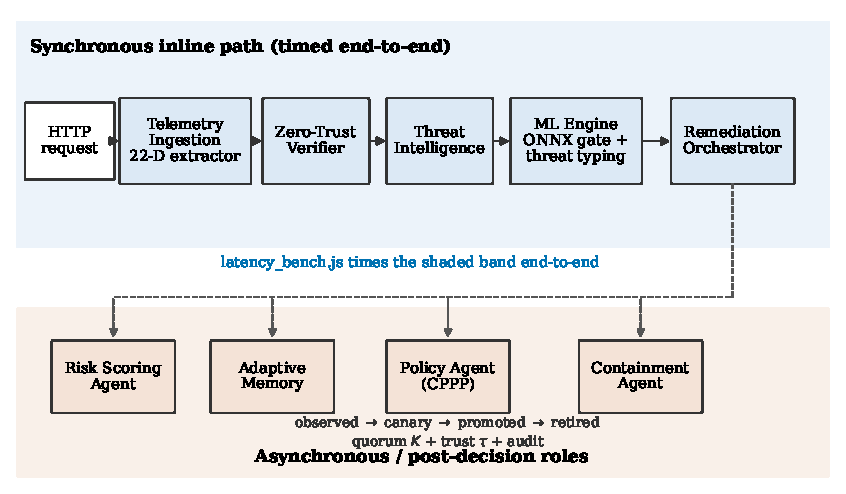
\includegraphics[width=4.9in,height=\textheight,keepaspectratio,alt={Figure 1. NATRIX architecture. The synchronous path contains five roles and produces the per-request verdict. The asynchronous band contains four governance roles; only the Policy Agent may promote a candidate, and promotion requires quorum, canary evidence, trust, and an audit record.}]{figures/architecture.pdf}
\caption{NATRIX architecture. The synchronous path contains
five roles and produces the per-request verdict. The asynchronous band
contains four governance roles; only the Policy Agent may promote a
candidate, and promotion requires quorum, canary evidence, trust, and an
audit record.}\label{fig:architecture}
\end{figure}

The asynchronous band contains \textbf{Risk Scoring} (per-session and
per-principal risk, which can raise a later request's risk but cannot
retroactively change a verdict), \textbf{Adaptive Memory} (incident
summaries, feature distributions, and drift indicators, off the decision
path), \textbf{Policy Agent} (CPPP: owns the candidate lifecycle, is the
only role allowed to promote or retire, and writes the audit record),
and \textbf{Containment} (post-decision side effects such as session
blocks, rule rollback, artifact quarantine, and operator notification).
Containment is outside the inline path because it may involve external
systems and cannot be bounded by the 5 ms reference. The paper evaluates
the gate as the primary learned component; the orchestration logic is
specified and unit-tested, and the headline accuracy numbers are gate
numbers.

The contract is computed from the method, path, query, body, and user
agent. It does not use response bodies, server logs, DNS, or external
reputation. The path is included deliberately: a WAF sees it, and
endpoint structure is real evidence. The paper therefore says
\emph{request contract}, not \emph{payload contract}. The lexical
baseline has a separate \emph{payload view} that excludes the path; that
view is a diagnostic, not a description of NATRIX.

The authority graph is acyclic with respect to promotion. Telemetry,
Zero-Trust, Threat Intelligence, and the ML Engine may submit evidence.
The Orchestrator may decide a request. Only the Policy Agent may change
the active policy, and it may not fabricate evidence; it consumes votes
and canary results produced by other roles. Containment may execute a
policy decision but may not create one. CPPP makes each of those
transitions impossible or explicit.

The adversary controls the HTTP request: method, path, query, headers,
body, encoding, and user agent, and may attempt SQL injection, XSS,
traversal, command injection, XXE, Log4Shell-style lookups, and
obfuscation. The base threat model assumes that agent processes, model
artifacts, and the audit log are not compromised, and that votes carry
authenticated agent identity. CPPP addresses unauthorised promotion by a
single agent and promotion without canary or quorum; it does not address
Byzantine collusion among a majority of agents, Sybil identities, model
poisoning, or supply-chain compromise. The evaluation is not an
adaptive-evasion study: the corpora were not generated by an adversary
who knows the feature set and threshold.

The current proxy implements the inline path and a simplified promotion
path. A new signature is inserted with \texttt{hit\allowbreak{}Count\ =\ 1}; the next
observation increments the count; the candidate becomes active when
\texttt{hitCount\ \textgreater{}=\ 2} or the source contains
\texttt{PCAP} or \texttt{Dataset}. There is no canary, independent
quorum, trust value, or automatic decay. That is exactly the transition
CPPP forbids, and the deployment audit below measures it on the live
deployment. Replacing the shortcut is the deployment step; the formal
results describe the specified protocol and its reference
implementation, not the shipped proxy.

\section{CPPP and trust decay}\label{cppp-and-trust-decay}

CPPP is a finite-state protocol for candidate rules and models. A
candidate has one of five states: observed, canary, promoted, retired,
or rejected. The allowed transitions are: observed -\textgreater{}
canary, when an independent quorum of at least \(K\) agents has voted
and trust is at least \(\tau\); canary -\textgreater{} promoted, only by
the Policy Agent, and only when the canary has passed, the quorum is
still present, and trust is at least \(\tau\); observed -\textgreater{}
rejected, by explicit policy decision; and promoted -\textgreater{}
retired, when trust falls below \(\tau\) on a scheduler tick. The canary
is an evidence event, not a free action: it requires at least \(N\)
observations, and none of them may be a benign hit. A hit is permanent,
so a candidate cannot be rescued by later clean traffic. There is no
observed -\textgreater{} promoted transition, no single-agent
vote-and-promote path, and no promotion without an audit record. Quorum
counts independent agent identities, not messages.

An earlier model coupled trust to votes: an agent gained trust by
voting, and quorum was counted over agents already above the floor. The
invariant was close to true by construction, and a mutant that removed
the quorum guard could survive. The revision adds a \texttt{Seed\allowbreak{}Trust}
action that sets trust independently of any vote. Votes are recorded
separately, and the promotion guard checks both, so a mutant that
removes the vote-count guard is killed even when trust is high.
\texttt{Seed\allowbreak{}Trust} is an environment assumption, not a model of how
trust is earned; it lets the model explore states in which an agent is
trusted but has not voted, or has voted but is not trusted.

TLC checks nine safety invariants: \texttt{Type\allowbreak{}OK};
\texttt{No\allowbreak{}Promotion\allowbreak{}Without\allowbreak{}Canary}; \texttt{No\allowbreak{}Promotion\allowbreak{}Without\allowbreak{}Quorum};
\texttt{No\allowbreak{}Promotion\allowbreak{}Without\allowbreak{}Trust};
\texttt{No\allowbreak{}Promotion\allowbreak{}Without\allowbreak{}Observations};
\texttt{No\allowbreak{}Promotion\allowbreak{}With\allowbreak{}Canary\allowbreak{}Hit}; \texttt{Active\allowbreak{}Implies\allowbreak{}Audited};
\texttt{Retired\allowbreak{}Not\allowbreak{}Active}; and \texttt{No\allowbreak{}Direct\allowbreak{}Promotion}. The two
observation invariants are the evidence coupling: a promoted rule must
have at least \(N\) observations and zero benign hits. These are safety,
not liveness, properties. The model proves that a bad transition cannot
occur, not that a good candidate will eventually be promoted.

Trust is a scalar in \([0,1]\). Without evidence it decays as
\(T(t) = T_0 e^{-\lambda t}\); positive evidence raises it towards 1
with gain \(\alpha \in (0,1]\). The implementation uses an exact
rational discrete model: one tick applies decay with factor
\(\rho \in (0,1)\), then reinforcement, so
\(\operatorname{tick}(T) = \rho T + \alpha(1-\rho T)\). Under stationary
evidence the fixed point is \(T^\ast = \alpha / (1-(1-\alpha)\rho)\) and
the closed form is \(T_n = T^\ast + (T_0 - T^\ast)((1-\alpha)\rho)^n\).
The contraction factor is strictly below 1, so the iteration converges
geometrically. A promoted rule whose trust falls below \(\tau\) is
retired atomically on the tick that would cross the floor; no observable
state has a promoted rule below \(\tau\).

The one-rule TLA+ configuration generates 939 states, 278 distinct, at
depth 12; the two-rule configuration generates 444,245 states, 77,284
distinct, at depth 23. Both report no error, and the nine invariants
hold. The executable reference is enumerated breadth-first to depth 9:
20,678 states and 97,870 transitions, with no violation, and 13 property
tests pass. The mutation test removes one guard at a time; all eight
mutants are killed (\texttt{no\_\allowbreak{}quorum}, \texttt{no\_\allowbreak{}canary},
\texttt{no\_\allowbreak{}trust}, \texttt{no\_\allowbreak{}audit}, \texttt{direct\_\allowbreak{}promote},
\texttt{retired\_\allowbreak{}active}, \texttt{canary\_\allowbreak{}hit},
\texttt{no\_\allowbreak{}observations}). Trust decay is checked on 17 trust points,
four decay factors, four gains, and 200 steps: 81,484 cases, zero
violations; nine symbolic identities are proved with SymPy. A sidecar
over 916 audit records verified the hash chain, matched 108 promotions
with 108 retirements (8 automatic), and held all eight runtime
invariants. Promotion and retirement cost 5.15 and 4.76 ms p95 without
fsync, and a full cycle 33.75 ms; fsync raises promotion and retirement
to 53.57 and 48.04 ms. Validation is heavier (45.82 ms p95, 522.41 ms
p99 under 32 parallel rules) and should be moved off the critical path.

\section{Feature admission}\label{feature-admission}

The runtime has four feature contracts: v1 (10-dimensional prototype),
v2 (16-dimensional threat typing), v3 (the 22-dimensional request
contract used by the binary gate), and v4 (the 20-dimensional contract
produced by admission). They share extraction code and differ only in
the mask; the ONNX export preserves input order. The 22 v3 features
cover shape, lexical counts and maxima, evasion scores, signature
scores, structural counts, and request-method risk. The names are
historical: \texttt{payload\_\allowbreak{}length}, \texttt{shannon\_\allowbreak{}entropy}, and the
ratio features are computed over the request target and body, not the
body alone. Header-coherence features were deferred by a frozen decision
(D1) because they would widen the contract beyond the fields the inline
proxy currently passes.

\subsection{Feature origin}\label{feature-origin}

v1 (10 features) was the first prototype, assembled from indicators
common in WAF rules and HTTP-anomaly work: request length, Shannon
entropy, character-class ratios, token count, SQL/XSS/traversal keyword
scores, and a scanner user-agent flag. v2 (16) added six features for
the threat-typing model: command-injection patterns, encoding ratio,
null-byte flag, duplicate-parameter count, HTML tag density, and
request-method risk. v3 (22) added six lexical features for the binary
gate: suspicious extensions, quote and angle counts, double escapes, and
maximum parameter-value ratio and length. The seven safety features come
from rules the runtime already enforced as direct policy signals. The v3
lexical block and the later candidate pool were shaped by error
inspection of gate misses, but the v1-to-v3 growth was iterative and not
frozen in advance; the admission procedure was introduced afterwards to
audit the result, and this paper reports that sequence. The full
formula, source field, and safety status of every feature are in
\texttt{tables/\allowbreak{}feature\_\allowbreak{}contract.\allowbreak{}csv} in the repository.

Admission is a decision procedure, not a search. A feature enters only
if it passes three gates in order, frozen before the v4 outcome is
inspected. \textbf{Gate A} requires the feature to be computable from
the request fields the inline proxy already has, deterministic, bounded
in cost, and independent of response bodies, logs, DNS, and external
reputation. It must not be on the frozen safety list: seven features are
retained because the runtime uses them as direct policy signals
(\texttt{sql\_\allowbreak{}keyword\_\allowbreak{}score}, \texttt{xss\_\allowbreak{}keyword\_\allowbreak{}score},
\texttt{path\_\allowbreak{}traversal\_\allowbreak{}score}, \texttt{command\_\allowbreak{}injection\_\allowbreak{}score},
\texttt{null\_\allowbreak{}byte\_\allowbreak{}score}, \texttt{request\_\allowbreak{}method\_\allowbreak{}risk}, and
\texttt{user\_\allowbreak{}agent\_\allowbreak{}anomaly}). Removing one from the model contract
would not remove the policy rule; it would only make the audit
misleading.

\textbf{Gate B} drops a feature only if all four conditions hold.
\textbf{C1 (univariate):} the Benjamini-Hochberg adjusted \(p\)-value
\citep{benjamini1995controlling} is at least 0.05 and the absolute
Cliff's delta is below 0.10, or the feature is near-constant. \textbf{C2
(importance):} permutation importance is in the bottom quartile and its
95\% bootstrap interval contains zero. \textbf{C3 (ablation):}
leave-one-feature-out ablation shows no degradation larger than the
practical-equivalence margin (0.2 percentage points of accuracy and 0.10
points of FPR). \textbf{C4 (safety):} the feature is not on the safety
list. The conjunction is conservative: a feature weak univariately but
important in the model is retained, and a statistically droppable safety
signal is retained.

\textbf{Gate C} requires the feature to fit the measured extraction
budget: added p95 cost on the 8 KiB worst case against a frozen 0.15 ms
budget. A feature that fails Gate C is not admitted even if Gate B
accepts it. The decision rule is
\(\operatorname{admit}(f) = \mathrm{Gate\,A}(f) \land \mathrm{Gate\,B}(f) \land \mathrm{Gate\,C}(f)\).
A feature is \emph{dropped} only if Gate A passes, Gate B fails, and it
is not on the safety list. A feature that passes Gate B but fails Gate C
is \emph{not admitted} but is not said to be statistically useless; the
distinction is recorded, and there is no post-hoc rescue.

Applied to the 22-dimensional v3 contract on CSIC 2010, the rule drops
exactly two features: \texttt{param\_\allowbreak{}pollution\_\allowbreak{}count} and
\texttt{html\_\allowbreak{}tag\_\allowbreak{}density}. Both are exactly zero in both classes, so
C1 holds by the near-constant clause, and their importance and ablation
are null. They are redundant dimensions, not signals removed because
they were inconvenient. Both are constant on this corpus, so the
evidence cannot show whether they carry signal elsewhere; they may. The
cross-corpus audit is descriptive and does not re-run selection (D10).
\texttt{token\_\allowbreak{}count} is the conservative case: its permutation
importance is -0.00054 with a 95\% interval of {[}-0.00082, -0.00026{]},
entirely below zero, so shuffling it slightly improves held-out
performance, but C2 requires the interval to contain zero, so the
feature is retained.

\texttt{special\_\allowbreak{}char\_\allowbreak{}ratio} is the more consequential anomaly. Its
univariate association is strong (BH-adjusted \(p \approx 10^{-180}\),
Cliff's \(\delta = 0.179\)), and its permutation importance is positive
(0.0831, rank 7 of 22), so C1 and C2 fail and the rule retains it. Yet
leave-one-out ablation shows that removing it \emph{improves} accuracy
by 1.52 percentage points (95\% CI {[}1.37, 1.68{]}) and lowers FPR by
0.24 points. C3 catches a harmful drop, not a beneficial removal, so it
does not reject the feature. The direction matches the cross-corpus
reversal: special-character density is higher in CSIC attacks but lower
in ECML and SR-BH attacks, so the forest learns a corpus-specific
direction. A post-hoc designer would drop it and report a 1.5-point
gain; we do not, because that decision would follow the outcome. The
1.52 points are an honest bound on what the frozen rule leaves on the
table.

The same mechanism screened 24 frozen candidates drawn from the
literature, runtime capability, and error analysis. Twelve pass the
statistical screen (mean delta F1 above its standard error and positive
in at least four of five folds). None is admitted. Gate C is applied to
the accepted block as a set, because the inline budget is an envelope
for the additional extraction pass, not a per-feature allowance. The
block costs 1.71 ms p95 on the 8 KiB worst case and 0.43 ms p95 on the
real CSIC distribution, against the 0.15 ms envelope; the full
24-candidate pass costs 2.33 ms. The counterfactual is therefore not
marginal: admitting the twelve statistically accepted candidates would
exceed the envelope by 11.4 times, and admitting all 24 by 15.5 times.
Table~\ref{tab:gate-c} gives the per-candidate marginal cost and the set-level budget.
Twenty candidates are individually below 0.15 ms. Even the nine accepted
candidates that are individually below budget cost 0.73 ms as a set,
because each shares a second parse.

The screen is not uniformly rejective. Table~\ref{tab:positive-control} is a positive control:
the four v3-D path features pass Gate B and Gate C, are admitted, and
change joint CSIC accuracy by +0.02 points. The procedure can admit a
candidate when the evidence supports it; the 24-candidate outcome is a
cost decision, not a prior against new features.

\textbf{How to add a feature.} The procedure is fixed before the
candidate is scored.

\begin{enumerate}
\def\labelenumi{\arabic{enumi}.}
\tightlist
\item
  Implement the feature in the Node and Python extractors with identical
  logic.
\item
  Gate A: use available request fields only; require deterministic,
  bounded cost.
\item
  Reject the feature if it is constant on the corpus or has
  \textbar Spearman\textbar{} $\ge$ 0.95 with an existing
  feature.
\item
  Add it to the 20-feature core; run the same five folds; accept only if
  the mean F1 gain exceeds its standard error and is positive in at
  least four of five folds.
\item
  Gate C: measure the whole accepted block's p95 cost on the 8 KiB worst
  case against the 0.15 ms budget.
\item
  Write the evidence row and the decision before looking at final test
  results.
\end{enumerate}



{
\begingroup\small
\begin{longtable}[]{@{}
  >{\raggedright\arraybackslash}p{(\linewidth - 6\tabcolsep) * \real{0.3400}}
  >{\raggedright\arraybackslash}p{(\linewidth - 6\tabcolsep) * \real{0.1600}}
  >{\raggedleft\arraybackslash}p{(\linewidth - 6\tabcolsep) * \real{0.2600}}
  >{\raggedright\arraybackslash}p{(\linewidth - 6\tabcolsep) * \real{0.2400}}@{}}
\caption{Gate C per-candidate cost and the set-level budget.
Marginal cost is the candidate's own extraction time on the 8 KiB
delimiter-heavy worst case, excluding the shared parse. The set rows
include the second parse because the candidate extractor is an
additional pass over the payload. The budget is 0.15 ms for the admitted
block.}\label{tab:gate-c}\\
\toprule\noalign{}
\begin{minipage}[t]{\linewidth}\raggedright
candidate
\end{minipage} & \begin{minipage}[t]{\linewidth}\raggedright
Gate B accepted
\end{minipage} & \begin{minipage}[t]{\linewidth}\raggedleft
marginal p95 (ms)
\end{minipage} & \begin{minipage}[t]{\linewidth}\raggedright
marginal $\le$ 0.15 ms
\end{minipage} \\
\midrule\noalign{}
\endfirsthead
\toprule\noalign{}
\begin{minipage}[t]{\linewidth}\raggedright
candidate
\end{minipage} & \begin{minipage}[t]{\linewidth}\raggedright
Gate B accepted
\end{minipage} & \begin{minipage}[t]{\linewidth}\raggedleft
marginal p95 (ms)
\end{minipage} & \begin{minipage}[t]{\linewidth}\raggedright
marginal $\le$ 0.15 ms
\end{minipage} \\
\midrule\noalign{}
\endhead
\bottomrule\noalign{}
\endlastfoot
\texttt{max\_\allowbreak{}param\_\allowbreak{}name\_\allowbreak{}entropy} & yes & 0.480 & no \\
\texttt{punctuation\_\allowbreak{}diversity} & no & 0.472 & no \\
\texttt{longest\_\allowbreak{}token\_\allowbreak{}length} & yes & 0.351 & no \\
\texttt{nonascii\_\allowbreak{}ratio} & yes & 0.257 & no \\
\texttt{param\_\allowbreak{}name\_\allowbreak{}digit\_\allowbreak{}ratio} & yes & 0.117 & yes \\
\texttt{ldap\_\allowbreak{}filter\_\allowbreak{}score} & yes & 0.014 & yes \\
\texttt{brace\_\allowbreak{}count} & yes & 0.013 & yes \\
\texttt{crlf\_\allowbreak{}sequence\_\allowbreak{}count} & yes & 0.008 & yes \\
\texttt{empty\_\allowbreak{}value\_\allowbreak{}ratio} & yes & 0.003 & yes \\
\texttt{url\_\allowbreak{}depth} & yes & 0.002 & yes \\
\end{longtable}
\endgroup
}

{\def\LTcaptype{none} % do not increment counter
\begingroup\small
\noindent\begin{tabular}{@{}
  >{\raggedright\arraybackslash}p{(\linewidth - 6\tabcolsep) * \real{0.3400}}
  >{\raggedright\arraybackslash}p{(\linewidth - 6\tabcolsep) * \real{0.1600}}
  >{\raggedleft\arraybackslash}p{(\linewidth - 6\tabcolsep) * \real{0.2600}}
  >{\raggedright\arraybackslash}p{(\linewidth - 6\tabcolsep) * \real{0.2400}}@{}}
\toprule
set & features & p95 (ms) & within 0.15 ms \\
\midrule
all candidates & 24 & 2.33 & no \\
Gate B accepted & 12 & 1.71 & no \\
accepted, marginal $\le$ 0.15 ms & 9 & 0.73 & no \\
\bottomrule
\end{tabular}
\endgroup
}

Selecting the cheap subset after inspecting this table would be the
post-hoc search the protocol forbids.



The nine v3-D features form two operational blocks. Gate C rejects the
five value features (0.35 ms p95 on the real CSIC distribution against
the 0.15 ms envelope) and accepts the four path features (0.085 ms).
Gate B is then applied to the path block. The full model is the 22-D v3
contract plus the four path features (26-D).

Full 26-D: 95.57\% accuracy, 1.92\% FPR, 92.63\% recall.

{
\begingroup\scriptsize\setlength{\tabcolsep}{2pt}
\begin{longtable}[]{@{}
  >{\raggedright\arraybackslash}p{(\linewidth - 10\tabcolsep) * \real{0.2600}}
  >{\raggedright\arraybackslash}p{(\linewidth - 10\tabcolsep) * \real{0.1000}}
  >{\raggedleft\arraybackslash}p{(\linewidth - 10\tabcolsep) * \real{0.1200}}
  >{\raggedleft\arraybackslash}p{(\linewidth - 10\tabcolsep) * \real{0.1200}}
  >{\raggedleft\arraybackslash}p{(\linewidth - 10\tabcolsep) * \real{0.2400}}
  >{\raggedleft\arraybackslash}p{(\linewidth - 10\tabcolsep) * \real{0.1600}}@{}}
\caption{Positive control: the four v3-D path features under
Gate B and Gate C. The full model is the 22-D v3 contract plus these
four features. All four are admitted; the joint CSIC accuracy change is
+0.02 percentage points.}\label{tab:positive-control}\\
\toprule\noalign{}
\begin{minipage}[t]{\linewidth}\raggedright
feature
\end{minipage} & \begin{minipage}[t]{\linewidth}\raggedleft
BH p
\end{minipage} & \begin{minipage}[t]{\linewidth}\raggedleft
Cliff delta
\end{minipage} & \begin{minipage}[t]{\linewidth}\raggedleft
perm. imp.
\end{minipage} & \begin{minipage}[t]{\linewidth}\raggedright
ablation delta acc. (95\% CI)
\end{minipage} & \begin{minipage}[t]{\linewidth}\raggedright
C1/C2/C3
\end{minipage} \\
\midrule\noalign{}
\endfirsthead
\toprule\noalign{}
\begin{minipage}[t]{\linewidth}\raggedright
feature
\end{minipage} & \begin{minipage}[t]{\linewidth}\raggedleft
BH p
\end{minipage} & \begin{minipage}[t]{\linewidth}\raggedleft
Cliff delta
\end{minipage} & \begin{minipage}[t]{\linewidth}\raggedleft
perm. imp.
\end{minipage} & \begin{minipage}[t]{\linewidth}\raggedright
ablation delta acc. (95\% CI)
\end{minipage} & \begin{minipage}[t]{\linewidth}\raggedright
C1/C2/C3
\end{minipage} \\
\midrule\noalign{}
\endhead
\bottomrule\noalign{}
\endlastfoot
\texttt{path\_\allowbreak{}special\_\allowbreak{}char\_\allowbreak{}ratio} & 9.3e-19 & +0.055 & +0.0314 &
+0.04pp {[}-0.11,+0.03{]} & no/no/yes \\
\texttt{path\_\allowbreak{}digit\_\allowbreak{}ratio} & 0.36 & -0.006 & +0.0016 & +0.02pp
{[}-0.09,+0.05{]} & yes/no/yes \\
\texttt{path\_\allowbreak{}uppercase\_\allowbreak{}ratio} & 2e-187 & +0.045 & -0.0000 & +0.04pp
{[}-0.10,+0.02{]} & no/yes/yes \\
\texttt{path\_\allowbreak{}keyword\_\allowbreak{}score} & 7e-05 & +0.001 & +0.0000 & -0.02pp
{[}-0.04,+0.09{]} & yes/no/yes \\
\end{longtable}
\endgroup
}

Gate C path-block p95: 0.085 ms (budget 0.15 ms). All four path features
are admitted. The joint accuracy change on CSIC is +0.02 percentage
points (95.57\% versus 95.55\%), so the admission is a procedural
positive control, not a claim of practical gain. The exercise is
post-freeze and does not change v4; it demonstrates that the gate is not
a reject-only procedure. The path signal matters on SR-BH, where the
view ablation shows that removing the path costs most of the recall.

The drop decision is made on CSIC only. The descriptive audit is
repeated on SR-BH 2020 and ECML/PKDD 2007 with one stratified 80/20
split per corpus, five permutation repeats, and full-corpus univariate
statistics with BH correction. This is a replication check, not a second
selection run (D10). Ten of the 22 features reverse direction on both
independent corpora, including \texttt{hex\_\allowbreak{}encoding\_\allowbreak{}ratio},
\texttt{payload\_\allowbreak{}length}, \texttt{special\_\allowbreak{}char\_\allowbreak{}ratio},
\texttt{sql\_\allowbreak{}keyword\_\allowbreak{}score}, and \texttt{quote\_\allowbreak{}count};
\texttt{uppercase\_\allowbreak{}ratio} is positive on CSIC (+0.298) and ECML (+0.243)
but strongly negative on SR-BH (-0.480). The direction of a feature is a
property of the corpus, application, and attack mix, not of the feature
name. The mechanism does not solve this; it produces a contract
defensible on the corpus where selection was made and reports the
reversal.

\section{Evaluation protocol}\label{evaluation-protocol}

Four labelled HTTP corpora are used. Table~\ref{tab:corpora} summarises their
composition, deduplication, and role. All are public or publicly
redistributable research corpora. No DNS logs, incident text, unlabelled
\texttt{http.\allowbreak{}log}, or production traffic is used for training or for any
accuracy claim. Sources and checksums are recorded in
\texttt{data/\allowbreak{}manifest.\allowbreak{}json}.



{
\begingroup\footnotesize\setlength{\tabcolsep}{3pt}
\begin{longtable}[]{@{}
  >{\raggedright\arraybackslash}p{(\linewidth - 10\tabcolsep) * \real{0.1600}}
  >{\raggedright\arraybackslash}p{(\linewidth - 10\tabcolsep) * \real{0.1900}}
  >{\raggedleft\arraybackslash}p{(\linewidth - 10\tabcolsep) * \real{0.0900}}
  >{\raggedleft\arraybackslash}p{(\linewidth - 10\tabcolsep) * \real{0.1400}}
  >{\raggedright\arraybackslash}p{(\linewidth - 10\tabcolsep) * \real{0.1300}}
  >{\raggedright\arraybackslash}p{(\linewidth - 10\tabcolsep) * \real{0.2900}}@{}}
\caption{Labelled HTTP corpora, deduplication, and split groups.
Counts are after exact deduplication and label-conflict removal. The
OpenAppSec WCP corpus is used only as an endpoint-matched diagnostic;
its random split is endpoint-confounded. It is never used for training
or model selection.}\label{tab:corpora}\\
\toprule\noalign{}
\begin{minipage}[t]{\linewidth}\raggedright
corpus
\end{minipage} & \begin{minipage}[t]{\linewidth}\raggedright
role
\end{minipage} & \begin{minipage}[t]{\linewidth}\raggedleft
records
\end{minipage} & \begin{minipage}[t]{\linewidth}\raggedleft
clean / attack
\end{minipage} & \begin{minipage}[t]{\linewidth}\raggedleft
groups
\end{minipage} & \begin{minipage}[t]{\linewidth}\raggedright
notes
\end{minipage} \\
\midrule\noalign{}
\endfirsthead
\toprule\noalign{}
\begin{minipage}[t]{\linewidth}\raggedright
corpus
\end{minipage} & \begin{minipage}[t]{\linewidth}\raggedright
role
\end{minipage} & \begin{minipage}[t]{\linewidth}\raggedleft
records
\end{minipage} & \begin{minipage}[t]{\linewidth}\raggedleft
clean / attack
\end{minipage} & \begin{minipage}[t]{\linewidth}\raggedleft
groups
\end{minipage} & \begin{minipage}[t]{\linewidth}\raggedright
notes
\end{minipage} \\
\midrule\noalign{}
\endhead
\bottomrule\noalign{}
\endlastfoot
CSIC 2010 & primary benchmark & 34,593 & 18,640 / 15,953 & endpoint
signatures & 97,065 raw; exact dedupe; 0 label conflicts \\
ECML 2007 & in-distribution & 50,116 & 35,006 / 15,110 & endpoint
signatures & official training set \\
SR-BH 2020 & in-distribution & 422,054 & 122,546 / 299,508 & 338,640 &
907,815 parsed; 485,237 duplicates; 524 conflicts removed \\
WCP 2024 & diagnostic only & 211,744 & 137,820 / 73,924 & 692 site files
& all malicious paths \texttt{/\allowbreak{}}; random split endpoint-confounded;
never trained or selected \\
\end{longtable}
\endgroup
}

CSIC 2010 \citep{csic2010dataset} is the primary in-distribution
benchmark. It is old and was generated against a small e-commerce
application; it is useful because its endpoint structure makes the P1/P2
distinction visible, not because it represents modern traffic. ECML/PKDD
2007 \citep{raissi2007web} is the classic challenge corpus, older than
CSIC and with a different label ontology; it is used as an
in-distribution corpus and as a transfer target. SR-BH 2020
\citep{srbh2020dataset} is the modern corpus; its attack-dominant prior
(299,508 attack vs 122,546 clean) is a property of the corpus, not a
deployment. The full corpus is used for the scale analysis in Section
7.5; the shared 20,000-request sample is used wherever a baseline must
be compared on identical rows. OpenAppSec WCP 2024
\citep{openappsec2024} supplies site-capped legitimate traffic and
malicious payloads; every malicious request has path \texttt{/\allowbreak{}}, so a
random split leaks the endpoint. WCP is never used for training or
threshold selection; the endpoint-matched subset (\texttt{path\ ==\ /\allowbreak{}})
is the diagnostic.

Duplicates are removed before splitting on (method, path, query, body,
user agent). A key that appears with two different labels is dropped and
counted.

\textbf{P1 (deployment-like)} is a stratified five-fold split over
unique requests. No identical request crosses the split, but the same
endpoint may appear in training and test. This is the headline protocol
because it matches WAF operation: the endpoint is known, and the
question is whether a request to it is malicious. \textbf{P2
(endpoint-disjoint)} is a stratified group five-fold split, where a
group is defined by (method, normalised path, query keys, body keys) and
assigned wholly to one fold. P2 is the generalisation bound, never the
headline number. It is not path-free: the path string remains a feature,
and what P2 removes is the identity of the endpoint as a memorisable
training item. The P2 folds are built once per corpus and reused by
every score-based detector, so the comparison is paired.

The primary learner is the shipped gate: a Random Forest
\citep{breiman2001random} with 200 trees, unlimited depth,
\texttt{min\_\allowbreak{}samples\_\allowbreak{}leaf=1}, \texttt{max\_\allowbreak{}features=None}, no class
weighting, and \texttt{random\_\allowbreak{}state=42}. It is pinned to the deployed
artifact (D5) and not tuned on test folds. The secondary learners are
histogram gradient boosting and L2-regularised logistic regression on
standardised features, both fixed untuned configurations (D9). All
learners use scikit-learn \citep{pedregosa2011scikit}, and the gate and
typing models are exported to ONNX and served with ONNX Runtime
\citep{onnxruntime2024}.

The generic control is a 17-feature LightGBM over request-shape
descriptors (method id, lengths, path depth, parameter counts,
body-to-URL ratio, character ratios, entropy, longest token, mean value
length, and has-query/has-body flags). It contains no SQL, XSS,
traversal, or scanner keyword score and no NATRIX feature, and uses the
same folds and 2\% policy. The cross-fitted stackers combine out-of-fold
scores with an L2 logistic model on logits; the stacker for fold \(k\)
is fitted on the other four folds and applied to fold \(k\). Three
stacks are reported: NATRIX+lexical, generic+lexical, and
NATRIX+generic+lexical.

Three threshold policies are reported: F1-optimal, FPR $\le$ 1\%,
and FPR $\le$ 2\%. The 2\% policy is the deployment point because
the acceptance target is FPR \textless{} 2.03\%; it was added after the
plan was frozen and is recorded as D8. The frozen protocol selects the
threshold by inner five-fold cross-validation inside each outer training
fold. That is the fully nested point, and it is conservative: inner
models see 64\% of the data while the scoring model sees 80\%, so the
probability scale differs. The cross-fitted calibration (D13) is a
sensitivity check: for each outer fold \(k\), the threshold is selected
on the outer out-of-fold predictions of the other four folds and applied
to fold \(k\). Fold \(k\)'s labels are never used to select its
threshold, but the models that score the other folds were trained on
data that includes fold \(k\), so this is a sensitivity analysis, not a
fully nested selection. The headline comparison uses the cross-fitted
2\% policy because every baseline can be calibrated the same way; the
fully nested result is reported for the primary corpus as the stricter
check.

\textbf{What ``pre-registered'' means here.} The analysis plan and
candidate pool were frozen on 2026-10-30 in the project repository
before the v4 screen and the matched-FPR comparison were run. This is a
project-level freeze, not a third-party preregistration: no OSF record
or public git history existed at freeze time. D8 (the 2\% operating
point) and D13 (cross-fitted calibration) were added after that freeze
and are recorded as deviations in \texttt{protocol/\allowbreak{}deviations.\allowbreak{}md}; the
headline 2\% comparison is therefore a post-freeze analysis, not a
confirmatory test. We use ``frozen'' in that limited sense and do not
claim that the entire analysis was preregistered.

Accuracy, FPR, FNR, precision, recall, F1, ROC-AUC, and PR-AUC are
reported. Confidence intervals are percentile bootstrap intervals with
2,000 resamples \citep{efron1993introduction}. Paired comparisons use
McNemar's test \citep{mcnemar1947note} and a paired bootstrap for the
accuracy difference; because several learners and corpora are compared,
we read individual tests as descriptive and do not apply a family-wise
correction \citep{demsar2006statistical}. The feature audit uses
Benjamini-Hochberg correction across the 22 tests. The three split seeds
are 42, 123, and 2026; the model's \texttt{random\_\allowbreak{}state} is fixed at 42
to match the shipped artifact.

The signature baseline is the official \texttt{owasp/\allowbreak{}modsecurity-crs}
4.25.2 nginx image at paranoia levels 1, 2, and 3, with the inbound
anomaly threshold at 5, request-body inspection on, and response-body
inspection off. The origin returns HTTP 200 for every request, so a 403
is the WAF decision. The replay sends the original method, path, query,
body, user agent, and content type as HTTP; no NATRIX feature extraction
is involved. Statuses 400, 405, 413, and 414 are nginx rejections that
occur before ModSecurity evaluates the request and are reported as
non-decisions. The full CSIC corpus is replayed at all three levels;
ECML, SR-BH, and WCP at PL1. The primary table uses decisions only.

The lexical baseline is a hashed character 2-4 gram representation
(\texttt{char\_\allowbreak{}wb}, \(2^{18}\) dimensions, L2-normalised) with an
L2-regularised logistic-loss SGD classifier, fixed at
\texttt{alpha=1e-5}, 30 epochs, and averaging. It is deliberately
simple, single-pass, and untuned: a strong reference, not a new model.
Three views are reported: \texttt{endpoint} (method and path),
\texttt{payload} (query and body), and \texttt{full} (path, query, and
body). The endpoint view tests whether a headline is an endpoint prior;
the payload view tests whether the signal survives without the path.
Thresholds are 0.5 and a leave-one-fold-out FPR $\le$ 2\%
threshold, identical to the NATRIX policy, and the P1/P2 lexical rows
use the same folds as NATRIX. An independent learned detector is also
run: a small character-level CNN (32-dimensional byte embedding, two
convolutional layers, max-pooling, five epochs) trained on the same
folds and calibrated with the same policy. It is a self-contained
reference, not a reproduction of a named system. Eight settings are
reported (CSIC and SR-BH, P1 and P2, full and payload views); Table~\ref{tab:matched-operating}
includes them.

The latency protocol measures the full inline decision: request
-\textgreater{} Node extraction -\textgreater{} HTTP \texttt{/\allowbreak{}predict}
-\textgreater{} ONNX gate -\textgreater{} threat typing -\textgreater{}
policy verdict. It uses the real Node proxy, Python service, and ONNX
artifacts, so it includes JSON serialisation, not just inference. The
input is 10,000 requests (5,000 CSIC, 3,000 ECML, 2,000 OpenAppSec);
after 300 warm-up requests, 9,700 are measured, and failures are
counted. The benchmark runs on one workstation (8 GB RAM, 12 logical
processors) with a single-process Python service. It excludes
synchronous SQLite writes, disk logging, and containment side effects,
and is a component measurement, not a throughput test; the 5 ms line in
Figure~\ref{fig:latency} is a reference point, not a pass/fail target.

\section{Results}\label{results}

\subsection{In-distribution accuracy and protocol
sensitivity}\label{in-distribution-accuracy-and-protocol-sensitivity}

Table~\ref{tab:matched-operating} reports the cross-fitted FPR $\le$ 2\% operating point used
throughout the paper.



\needspace{9\baselineskip}
\textbf{Panel A: P1 (deployment-like, endpoint may recur)}

{
\begingroup\scriptsize\setlength{\tabcolsep}{3pt}
\begin{longtable}[]{@{}
  >{\raggedright\arraybackslash}p{(\linewidth - 10\tabcolsep) * \real{0.1667}}
  >{\raggedright\arraybackslash}p{(\linewidth - 10\tabcolsep) * \real{0.1667}}
  >{\raggedleft\arraybackslash}p{(\linewidth - 10\tabcolsep) * \real{0.1667}}
  >{\raggedleft\arraybackslash}p{(\linewidth - 10\tabcolsep) * \real{0.1667}}
  >{\raggedleft\arraybackslash}p{(\linewidth - 10\tabcolsep) * \real{0.1667}}
  >{\raggedleft\arraybackslash}p{(\linewidth - 10\tabcolsep) * \real{0.1667}}@{}}
\caption{Matched operating points at the cross-fitted FPR
$\le$ 2\% policy. All score-based detectors use leave-one-fold-out
thresholds; CRS is a frozen ModSecurity CRS 4.25.2 PL1 replay and is not
tuned to a 2\% budget. The generic control is a 17-feature LightGBM
trained on the same folds; the stacks are cross-fitted logistic
combinations of the listed base scores; CNN is an independent
character-level convolutional detector trained on the same folds and
calibrated with the same policy. SR-BH rows use the shared
20,000-request sample. Values are percentages.}\label{tab:matched-operating}\\
\toprule\noalign{}
corpus & detector & accuracy & FPR & recall & F1 \\
\midrule\noalign{}
\endfirsthead
\toprule\noalign{}
corpus & detector & accuracy & FPR & recall & F1 \\
\midrule\noalign{}
\endhead
\bottomrule\noalign{}
\endlastfoot
CSIC & NATRIX & 95.55 & 1.93 & 92.60 & 0.9505 \\
CSIC & Lex-full & 96.57 & 1.96 & 94.84 & 0.9622 \\
CSIC & Lex-payload & 96.90 & 1.88 & 95.47 & 0.9660 \\
CSIC & Lex-endpt & 60.85 & 0.14 & 15.26 & 0.2645 \\
CSIC & CNN-full & 96.47 & 1.28 & 93.84 & 0.9608 \\
CSIC & CNN-payload & 96.58 & 1.02 & 93.79 & 0.9620 \\
CSIC & CRS PL1 & 66.24 & 0.03 & 26.84 & 0.4230 \\
CSIC & Generic GBM & 86.90 & 1.97 & 73.90 & 0.8388 \\
CSIC & Stack NATRIX+Lex & 98.45 & 1.24 & 98.08 & 0.9831 \\
CSIC & Stack N+G+Lex & 98.44 & 1.24 & 98.08 & 0.9831 \\
ECML & NATRIX & 91.96 & 1.67 & 77.19 & 0.8527 \\
ECML & Lex-full & 93.93 & 0.43 & 80.85 & 0.8893 \\
ECML & Lex-payload & 92.66 & 0.54 & 76.90 & 0.8633 \\
ECML & Lex-endpt & 71.94 & 1.80 & 11.11 & 0.1927 \\
ECML & CRS PL1 & 78.64 & 20.13 & 75.70 & 0.6752 \\
SR-BH & NATRIX (20k) & 90.79 & 1.96 & 87.82 & 0.9312 \\
SR-BH & Lex-full & 95.41 & 1.98 & 94.34 & 0.9668 \\
SR-BH & Lex-payload & 36.20 & 2.00 & 10.91 & 0.1954 \\
SR-BH & CNN-full & 95.34 & 2.36 & 94.41 & 0.9664 \\
SR-BH & CNN-payload & 36.05 & 1.95 & 10.67 & 0.1915 \\
SR-BH & CRS PL1 & 44.29 & 25.80 & 32.00 & 0.4488 \\
\end{longtable}
\endgroup
}

\needspace{9\baselineskip}
\textbf{Panel B: P2 (endpoint-disjoint, unseen endpoint groups)}

{\def\LTcaptype{none} % do not increment counter
\begingroup\scriptsize\setlength{\tabcolsep}{3pt}
\noindent\begin{tabular}{@{}
  >{\raggedright\arraybackslash}p{(\linewidth - 10\tabcolsep) * \real{0.1667}}
  >{\raggedright\arraybackslash}p{(\linewidth - 10\tabcolsep) * \real{0.1667}}
  >{\raggedleft\arraybackslash}p{(\linewidth - 10\tabcolsep) * \real{0.1667}}
  >{\raggedleft\arraybackslash}p{(\linewidth - 10\tabcolsep) * \real{0.1667}}
  >{\raggedleft\arraybackslash}p{(\linewidth - 10\tabcolsep) * \real{0.1667}}
  >{\raggedleft\arraybackslash}p{(\linewidth - 10\tabcolsep) * \real{0.1667}}@{}}
\toprule
corpus & detector & accuracy & FPR & recall & F1 \\
\midrule
CSIC & NATRIX & 78.85 & 6.50 & 61.73 & 0.7291 \\
CSIC & Lex-full & 69.53 & 21.57 & 59.13 & 0.6415 \\
CSIC & Lex-payload & 96.03 & 2.43 & 94.24 & 0.9564 \\
CSIC & Lex-endpt & 51.55 & 21.50 & 20.05 & 0.2763 \\
CSIC & CNN-full & 85.45 & 21.63 & 93.72 & 0.8559 \\
CSIC & CNN-payload & 96.03 & 1.57 & 93.23 & 0.9559 \\
CSIC & Generic GBM & 67.65 & 30.80 & 65.84 & 0.6525 \\
CSIC & Stack NATRIX+Lex & 67.55 & 21.35 & 54.57 & 0.6080 \\
CSIC & Stack N+G+Lex & 72.71 & 21.07 & 65.43 & 0.6886 \\
ECML & NATRIX & 91.60 & 1.75 & 76.21 & 0.8455 \\
ECML & Lex-full & 93.76 & 0.51 & 80.47 & 0.8860 \\
ECML & Lex-payload & 92.70 & 0.44 & 76.81 & 0.8638 \\
ECML & Lex-endpt & 71.79 & 1.97 & 11.00 & 0.1904 \\
ECML & Generic GBM & 90.74 & 1.90 & 73.69 & 0.8275 \\
ECML & Stack NATRIX+Lex & 94.02 & 0.35 & 80.99 & 0.8909 \\
ECML & Stack N+G+Lex & 93.91 & 0.51 & 80.97 & 0.8891 \\
SR-BH & NATRIX (20k) & 90.62 & 1.88 & 87.56 & 0.9299 \\
SR-BH & Lex-full & 94.75 & 2.01 & 93.43 & 0.9619 \\
SR-BH & Lex-payload & 36.27 & 1.88 & 10.97 & 0.1964 \\
SR-BH & Lex-endpt & 93.08 & 2.08 & 91.11 & 0.9492 \\
SR-BH & CNN-full & 95.28 & 1.86 & 94.10 & 0.9658 \\
SR-BH & CNN-payload & 41.63 & 19.01 & 25.53 & 0.3831 \\
\bottomrule
\end{tabular}
\endgroup
}

Under P1, NATRIX reaches 95.55/1.93 on CSIC, 91.96/1.67 on ECML, and
90.79/1.96 on the SR-BH 20k sample. The lexical full-request baseline is
stronger than NATRIX on every corpus at the same policy: 96.57/1.96,
93.93/0.43, and 95.41/1.98, and the independent char-CNN is comparable
on CSIC (96.47/1.28 full, 96.58/1.02 payload). The lexical payload view
is also stronger on CSIC and ECML (96.90/1.88 and 92.66/0.54) but
collapses on SR-BH (36.20/2.00, 10.91\% recall). CRS PL1 is not
competitive (Table~\ref{tab:matched-operating}).

The P2 panel changes the ranking. NATRIX falls to 78.85/6.50 on CSIC,
91.60/1.75 on ECML, and 90.62/1.88 on SR-BH. Lexical full falls from
96.57\% to 69.53\% on CSIC and its FPR rises from 1.96\% to 21.57\%,
while lexical payload stays at 96.03/2.43 with 94.24\% recall. The
full-request model was using endpoint identity; on unseen endpoints that
prior becomes a false-positive generator. NATRIX falls less in accuracy
than lexical full, but its FPR rises from 1.93\% to 6.50\% and its
recall falls from 92.60\% to 61.73\%. It is more robust than lexical
full but not competitive with lexical payload, the strongest CSIC P2
detector.

The SR-BH P2 row tells the opposite story. Lexical full stays at
94.75/2.01 with 93.43\% recall, and lexical payload collapses to
36.27/1.88 with 10.97\% recall. The path is the signal on SR-BH, and it
generalises to unseen groups. NATRIX is 90.62/1.88 with 87.56\% recall,
below lexical full.

The independent char-CNN reproduces the inversion: on CSIC its full view
collapses from 96.47/1.28 under P1 to 85.45/21.63 under P2 while payload
holds at 96.03/1.57; on SR-BH full stays at 95.34/2.36 and 95.28/1.86
while payload falls to 36.05/1.95 and 41.63/19.01. The collapse is a
property of the protocol and the view, not of the learner.

A P1-only paper would conclude that the lexical baseline is the best
single detector on every corpus; a P2-only paper would conclude that
lexical payload is best on CSIC and lexical full on SR-BH. Neither
summary is universal: the ranking is protocol- and corpus-dependent.
Figure~\ref{fig:protocol} plots the operating points.

\begin{figure}
\centering
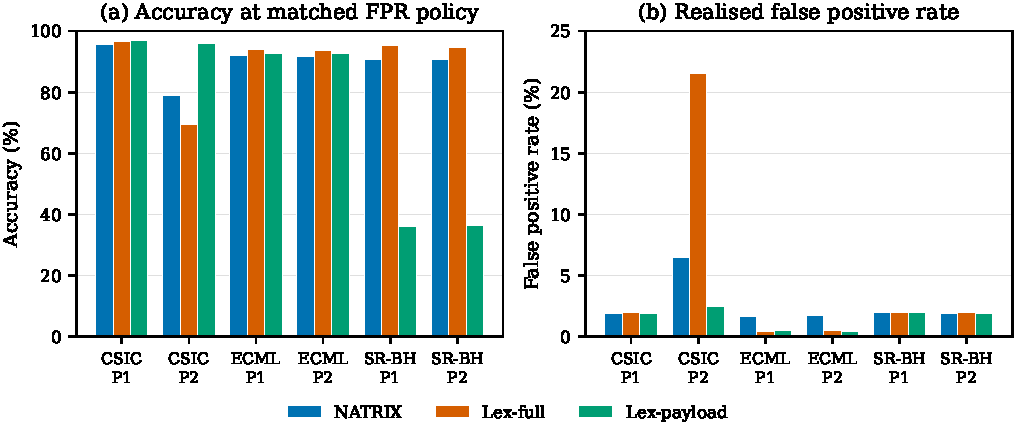
\includegraphics[width=4.9in,height=\textheight,keepaspectratio,alt={Figure 2. Matched operating points for NATRIX, the lexical full-request baseline, and the lexical payload baseline under P1 and P2. Panel (a) is accuracy and panel (b) is the realised false positive rate. The CSIC P2 panel shows the endpoint-disjoint collapse of the full-request lexical model; the SR-BH P2 panel shows the opposite payload collapse. All values are from Table 4.}]{figures/revision_protocol_sensitivity.pdf}
\caption{Matched operating points for NATRIX, the lexical
full-request baseline, and the lexical payload baseline under P1 and P2.
Panel (a) is accuracy and panel (b) is the realised false positive rate.
The CSIC P2 panel shows the endpoint-disjoint collapse of the
full-request lexical model; the SR-BH P2 panel shows the opposite
payload collapse. All values are from Table~\ref{tab:matched-operating}.}\label{fig:protocol}
\end{figure}

The fully nested check adds a caveat. On CSIC P1, the inner-CV FPR
$\le$ 2\% policy selects thresholds around 0.57 and yields 94.67\%
accuracy at 1.26\% FPR for v3, and 94.59\% at 1.24\% for v4: 0.33 to
0.41 points below the 95\% target. The cross-fitted policy selects
thresholds around 0.51 and yields 95.55\% at about 1.95\% FPR; the gap
is a threshold-scale artifact.

\subsection{View ablation: where the signal
is}\label{view-ablation-where-the-signal-is}

Table~\ref{tab:view-ablation} reports five views of the same 22-dimensional contract across
six corpus-protocol groups: full, no-path, path-only, query-only, and
body-only. All rows use the same folds and the same cross-fitted FPR
$\le$ 2\% policy.



{
\begingroup\scriptsize\setlength{\tabcolsep}{3pt}
\begin{longtable}[]{@{}
  >{\raggedright\arraybackslash}p{(\linewidth - 12\tabcolsep) * \real{0.1429}}
  >{\raggedright\arraybackslash}p{(\linewidth - 12\tabcolsep) * \real{0.1429}}
  >{\raggedright\arraybackslash}p{(\linewidth - 12\tabcolsep) * \real{0.1429}}
  >{\raggedleft\arraybackslash}p{(\linewidth - 12\tabcolsep) * \real{0.1429}}
  >{\raggedleft\arraybackslash}p{(\linewidth - 12\tabcolsep) * \real{0.1429}}
  >{\raggedleft\arraybackslash}p{(\linewidth - 12\tabcolsep) * \real{0.1429}}
  >{\raggedleft\arraybackslash}p{(\linewidth - 12\tabcolsep) * \real{0.1429}}@{}}
\caption{View ablation. \texttt{full} is the 22-D request
contract (method, path, query, body, user agent). \texttt{no\_\allowbreak{}path}
removes every path-derived feature. \texttt{path\_\allowbreak{}only} retains only
path-derived features. \texttt{query\_\allowbreak{}only} and \texttt{body\_\allowbreak{}only}
retain the corresponding lexical/structural features. All rows use the
same P1 or P2 folds and the cross-fitted FPR $\le$ 2\% policy. CSIC
is reported under both protocols so that the P2 path-only collapse can
be read against its P1 control. Values are percentages.}\label{tab:view-ablation}\\
\toprule\noalign{}
corpus & protocol & view & accuracy & FPR & recall & F1 \\
\midrule\noalign{}
\endfirsthead
\toprule\noalign{}
corpus & protocol & view & accuracy & FPR & recall & F1 \\
\midrule\noalign{}
\endhead
\bottomrule\noalign{}
\endlastfoot
SR-BH 20k & P1 & full & 90.79 & 1.96 & 87.82 & 0.9312 \\
SR-BH 20k & P1 & no\_path & 37.52 & 1.93 & 12.74 & 0.2244 \\
SR-BH 20k & P1 & path\_only & 89.16 & 1.98 & 85.53 & 0.9180 \\
SR-BH 20k & P1 & query\_only & 36.35 & 1.91 & 11.10 & 0.1984 \\
SR-BH 20k & P1 & body\_only & 35.38 & 1.55 & 9.58 & 0.1739 \\
SR-BH 20k & P2 & full & 90.62 & 1.88 & 87.56 & 0.9299 \\
SR-BH 20k & P2 & no\_path & 37.29 & 2.08 & 12.49 & 0.2203 \\
SR-BH 20k & P2 & path\_only & 89.05 & 1.83 & 85.31 & 0.9170 \\
SR-BH 20k & P2 & query\_only & 34.03 & 1.55 & 7.68 & 0.1418 \\
SR-BH 20k & P2 & body\_only & 35.24 & 1.86 & 9.50 & 0.1724 \\
CSIC & P1 & full & 95.55 & 1.93 & 92.60 & 0.9505 \\
CSIC & P1 & no\_path & 95.34 & 2.01 & 92.24 & 0.9481 \\
CSIC & P1 & path\_only & 60.87 & 0.09 & 15.26 & 0.2645 \\
CSIC & P1 & query\_only & 73.26 & 1.98 & 44.34 & 0.6047 \\
CSIC & P1 & body\_only & 68.77 & 2.00 & 34.62 & 0.5056 \\
CSIC & P2 & full & 78.85 & 6.50 & 61.73 & 0.7291 \\
CSIC & P2 & no\_path & 75.07 & 4.26 & 50.92 & 0.6532 \\
CSIC & P2 & path\_only & 34.47 & 99.92 & 74.64 & 0.5123 \\
CSIC & P2 & query\_only & 51.02 & 27.27 & 25.66 & 0.3258 \\
CSIC & P2 & body\_only & 50.45 & 28.06 & 25.34 & 0.3205 \\
\end{longtable}
\endgroup
}

On SR-BH, the full model reaches 90.79/1.96 with 87.82\% recall under
P1, and 90.62/1.88 with 87.56\% recall under P2. Removing the path drops
recall to 12.74\% (P1) and 12.49\% (P2). A path-only model retains
85.53\% (P1) and 85.31\% (P2), nearly the full model. Query-only and
body-only models are weak (11.10\% and 9.58\% recall under P1). The path
carries almost all of the SR-BH signal. This is not endpoint
memorisation, because it survives P2: the path morphology itself
(traversal sequences, encoded SQL, suspicious extensions) separates the
classes. But it means SR-BH is not evidence for payload detection, and
the lexical payload collapse is consistent with that reading. Figure~\ref{fig:views}
plots the five views.

On CSIC P2, the pattern inverts. The full model reaches 78.85/6.50 with
61.73\% recall. Removing the path gives 75.07/4.26 with 50.92\% recall:
only 3.78 points below full accuracy, with a lower FPR. A path-only
model has high recall (74.64\%) but flags 99.92\% of clean requests, so
accuracy collapses to 34.47\%. Query-only and body-only models are
individually weak (51.02\% and 50.45\% accuracy), but together, as
\texttt{no\_\allowbreak{}path}, they reach 75.07\%. On CSIC P2 the path adds recall
at a false-positive cost, and the payload features carry substantial
signal.

The CSIC P1 rows are the control that separates two readings of that
collapse. Under P1 the full model reaches 95.55/1.93 with 92.60\%
recall, and removing the path changes nothing material: 95.34/2.01 with
92.24\% recall, a 0.21-point accuracy difference. Path-only reaches
60.87\% accuracy with 15.26\% recall at 0.09\% FPR, and query-only alone
recovers 44.34\% recall. The CSIC P1 headline is therefore not a path
prior; it is payload signal. Yet the same path-only model that flags
0.09\% of clean requests under P1 flags 99.92\% under P2. That flip is a
threshold-transfer failure, not a change in what the path contains:
path-derived scores are nearly degenerate, so a small shift on unseen
endpoints moves almost every clean request across a threshold calibrated
at 2\% on seen ones. The endpoint prior on CSIC is not the path string
but endpoint-conditioned payload statistics, which is consistent with
the full model's FPR rising from 1.93\% to 6.50\% under P2 while lexical
payload, which pools n-grams across endpoints, stays at 2.43\%.

\begin{figure}
\centering
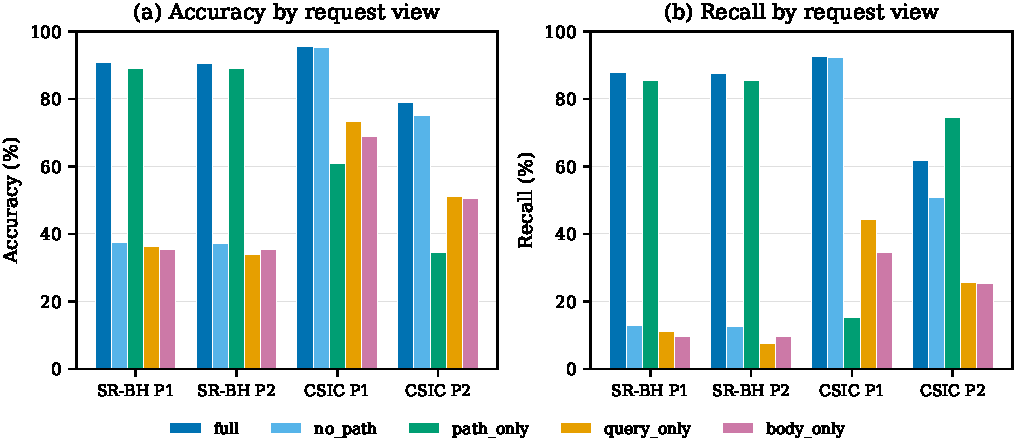
\includegraphics[width=4.9in,height=\textheight,keepaspectratio,alt={Figure 3. View ablation for the 22-D contract. Panel (a) is accuracy and panel (b) is recall for the full, no-path, path-only, query-only, and body-only views. On SR-BH the path carries almost all of the signal under both protocols; on CSIC P2 the path-only model collapses to 34.47\% accuracy because it flags 99.92\% of clean requests, while the same model under CSIC P1 flags 0.09\%. All values are from Table 5.}]{figures/revision_view_ablation.pdf}
\caption{View ablation for the 22-D contract. Panel (a) is
accuracy and panel (b) is recall for the full, no-path, path-only,
query-only, and body-only views. On SR-BH the path carries almost all of
the signal under both protocols; on CSIC P2 the path-only model
collapses to 34.47\% accuracy because it flags 99.92\% of clean
requests, while the same model under CSIC P1 flags 0.09\%. All values
are from Table~\ref{tab:view-ablation}.}\label{fig:views}
\end{figure}

This answers the ``NATRIX versus payload-only'' inconsistency. NATRIX is
a request-level contract, and the ablation shows what each view
contributes. On CSIC P2, lexical payload is stronger than full NATRIX;
on SR-BH P2, full NATRIX is stronger because the path signal is real.
The paper does not claim payload-only detection.

The CSIC P2 operating point is also a failure against the paper's own
target: 6.50\% FPR is above 2\%, and even the no-path view is at 4.26\%.
The threshold selected on training folds at 2\% does not hold on unseen
endpoints. This is a limitation of the calibration protocol, not a
threshold-tuning problem: no single threshold can fix a ranking that
changes with the endpoint population.

\subsection{Is the ranking change larger than sampling
noise?}\label{is-the-ranking-change-larger-than-sampling-noise}

The tables report point estimates; the claim is that the change in
ranking is larger than sampling noise. We bootstrap the paired
difference-in-differences over requests, using the same out-of-fold
predictions and the same leave-one-fold-out thresholds as Table~\ref{tab:matched-operating}, with
2,000 resamples. The script asserts that the recomputed point estimates
reproduce Table~\ref{tab:matched-operating} before it bootstraps, and writes the full grid to
\texttt{protocol\_\allowbreak{}interaction.\allowbreak{}json} in the artifact.

The NATRIX-minus-lexical-full gap moves by +10.33 points on CSIC between
P1 and P2 (95\% CI {[}9.72, 10.96{]}): NATRIX is 1.02 points behind
under P1 and 9.32 ahead under P2. On ECML the same quantity is -0.19
points ({[}-0.30, -0.07{]}) and on SR-BH +0.49 ({[}0.18, 0.80{]}), so
the protocol change alone does not reorder the ranking on those corpora;
the intervals exclude zero but the effects are negligible. The view
effect is where the corpora separate: payload-minus-full moves by +26.17
points on CSIC ({[}25.66, 26.67{]}) but only +0.73 on SR-BH ({[}0.52,
0.94{]}) and +0.21 on ECML ({[}0.14, 0.28{]}). The 25.4-point difference
between the CSIC and SR-BH view interactions is the quantitative form of
the paper's central claim: the value of the path is a property of the
corpus, and the endpoint-disjoint protocol exposes it on CSIC without
creating it on SR-BH. The resampling unit is the request, matching the
intervals reported elsewhere; it does not model fold-level variance, so
the intervals describe request-level uncertainty only.

\subsection{Control models and
stackers}\label{control-models-and-stackers}

Table~\ref{tab:control-models} reports the generic control and the cross-fitted stackers. The
generic control is weaker than NATRIX on every corpus at the same FPR
budget, most clearly on CSIC P1 (73.90 versus 92.60 recall) and SR-BH P2
(61.30 versus 87.56).



{
\begingroup\scriptsize\setlength{\tabcolsep}{3pt}
\begin{longtable}[]{@{}
  >{\raggedright\arraybackslash}p{(\linewidth - 12\tabcolsep) * \real{0.1154}}
  >{\raggedright\arraybackslash}p{(\linewidth - 12\tabcolsep) * \real{0.1154}}
  >{\raggedleft\arraybackslash}p{(\linewidth - 12\tabcolsep) * \real{0.1538}}
  >{\raggedleft\arraybackslash}p{(\linewidth - 12\tabcolsep) * \real{0.1538}}
  >{\raggedleft\arraybackslash}p{(\linewidth - 12\tabcolsep) * \real{0.1538}}
  >{\raggedleft\arraybackslash}p{(\linewidth - 12\tabcolsep) * \real{0.1538}}
  >{\raggedleft\arraybackslash}p{(\linewidth - 12\tabcolsep) * \real{0.1538}}@{}}
\caption{Generic control and cross-fitted stackers. Cells are
accuracy/FPR (\%). The generic control is a 17-feature LightGBM over
request-shape, lexical, and method features that are not the NATRIX
contract. The stackers combine out-of-fold scores with a logistic model
fitted on the other four folds; the threshold is selected
leave-one-fold-out at FPR $\le$ 2\%. \texttt{Lex} is the hashed
character n-gram baseline in the stated view.}\label{tab:control-models}\\
\toprule\noalign{}
\begin{minipage}[t]{\linewidth}\raggedright
corpus
\end{minipage} & \begin{minipage}[t]{\linewidth}\raggedright
view
\end{minipage} & \begin{minipage}[t]{\linewidth}\raggedleft
NATRIX
\end{minipage} & \begin{minipage}[t]{\linewidth}\raggedleft
Lex
\end{minipage} & \begin{minipage}[t]{\linewidth}\raggedleft
Generic
\end{minipage} & \begin{minipage}[t]{\linewidth}\raggedleft
N+Lex
\end{minipage} & \begin{minipage}[t]{\linewidth}\raggedleft
N+G+Lex
\end{minipage} \\
\midrule\noalign{}
\endfirsthead
\toprule\noalign{}
\begin{minipage}[t]{\linewidth}\raggedright
corpus
\end{minipage} & \begin{minipage}[t]{\linewidth}\raggedright
view
\end{minipage} & \begin{minipage}[t]{\linewidth}\raggedleft
NATRIX
\end{minipage} & \begin{minipage}[t]{\linewidth}\raggedleft
Lex
\end{minipage} & \begin{minipage}[t]{\linewidth}\raggedleft
Generic
\end{minipage} & \begin{minipage}[t]{\linewidth}\raggedleft
N+Lex
\end{minipage} & \begin{minipage}[t]{\linewidth}\raggedleft
N+G+Lex
\end{minipage} \\
\midrule\noalign{}
\endhead
\bottomrule\noalign{}
\endlastfoot
CSIC P1 & full & 95.55/1.93 & 96.57/1.96 & 86.90/1.97 & 98.45/1.24 &
98.44/1.24 \\
CSIC P2 & full & 78.85/6.50 & 69.53/21.57 & 67.65/30.80 & 67.55/21.35 &
72.71/21.07 \\
CSIC P2 & payload & 78.85/6.50 & 96.03/2.43 & 67.65/30.80 & 95.89/2.70 &
96.33/1.85 \\
ECML P2 & full & 91.60/1.75 & 93.76/0.51 & 90.74/1.90 & 94.02/0.35 &
93.91/0.51 \\
ECML P2 & payload & 91.60/1.75 & 92.70/0.44 & 90.74/1.90 & 93.54/0.40 &
93.63/0.74 \\
SR-BH 20k P2 & full & 90.62/1.88 & 94.75/2.01 & 71.96/2.00 & 96.21/2.00
& 96.19/2.01 \\
SR-BH 20k P2 & payload & 90.62/1.88 & 36.27/1.88 & 71.96/2.00 &
91.46/1.95 & 91.64/2.00 \\
\end{longtable}
\endgroup
}

Cells are accuracy/FPR (\%). \texttt{Lex} is the hashed character n-gram
baseline in the stated view. The NATRIX score is the same 22-D model in
both payload rows, because the contract always includes the path.

The stackers show where fusion helps and where it does not. On CSIC P1,
NATRIX+lexical improves on lexical by +1.88 points (95\% CI {[}1.71,
2.04{]}) and on generic+lexical by +1.47 points. On SR-BH P2 full, the
gains are +1.46 and +2.60 points. On ECML P2 full the gain is +0.26
points; on ECML P2 payload it is +0.85. On CSIC P2 full, the
NATRIX+lexical stack is worse than lexical alone by -1.98 points; on
CSIC P2 payload it is -0.14. The full stack inherits both base scores'
endpoint failure, and the payload stack is essentially tied with lexical
payload.

The SR-BH P2 payload row is a special case. NATRIX+lexical reaches
91.46/1.95 versus lexical payload 36.27/1.88, a +55.18-point gain. That
is not fusion recovering payload signal; it is the NATRIX path signal
re-entering the stack. The +18.72-point gain of NATRIX+generic+lexical
over generic+lexical is the value of that path signal. On CSIC P2
payload, where the path signal is harmful, the NATRIX score adds
nothing: -0.30 points versus generic+lexical.

\subsection{Grouping sensitivity}\label{grouping-sensitivity}

The P2 split groups requests by method, normalised path, and sorted
query and body parameter names. We rebuilt the folds with path-only
groups, which is stricter because requests to the same path with
different parameter names can no longer be separated. Table~\ref{tab:grouping} reports
the check.



{
\begingroup\scriptsize\setlength{\tabcolsep}{3pt}
\begin{longtable}[]{@{}
  >{\raggedright\arraybackslash}p{(\linewidth - 10\tabcolsep) * \real{0.1429}}
  >{\raggedright\arraybackslash}p{(\linewidth - 10\tabcolsep) * \real{0.1429}}
  >{\raggedleft\arraybackslash}p{(\linewidth - 10\tabcolsep) * \real{0.1905}}
  >{\raggedleft\arraybackslash}p{(\linewidth - 10\tabcolsep) * \real{0.1905}}
  >{\raggedleft\arraybackslash}p{(\linewidth - 10\tabcolsep) * \real{0.1905}}
  >{\raggedright\arraybackslash}p{(\linewidth - 10\tabcolsep) * \real{0.1429}}@{}}
\caption{P2 grouping sensitivity under path-only groups. Values
are percentages.}\label{tab:grouping}\\
\toprule\noalign{}
\begin{minipage}[t]{\linewidth}\raggedright
corpus
\end{minipage} & \begin{minipage}[t]{\linewidth}\raggedright
grouping
\end{minipage} & \begin{minipage}[t]{\linewidth}\raggedleft
groups
\end{minipage} & \begin{minipage}[t]{\linewidth}\raggedleft
max group
\end{minipage} & \begin{minipage}[t]{\linewidth}\raggedleft
rows in mixed groups
\end{minipage} & \begin{minipage}[t]{\linewidth}\raggedright
balanced 5-fold?
\end{minipage} \\
\midrule\noalign{}
\endfirsthead
\toprule\noalign{}
\begin{minipage}[t]{\linewidth}\raggedright
corpus
\end{minipage} & \begin{minipage}[t]{\linewidth}\raggedright
grouping
\end{minipage} & \begin{minipage}[t]{\linewidth}\raggedleft
groups
\end{minipage} & \begin{minipage}[t]{\linewidth}\raggedleft
max group
\end{minipage} & \begin{minipage}[t]{\linewidth}\raggedleft
rows in mixed groups
\end{minipage} & \begin{minipage}[t]{\linewidth}\raggedright
balanced 5-fold?
\end{minipage} \\
\midrule\noalign{}
\endhead
\bottomrule\noalign{}
\endlastfoot
CSIC & endpoint + params & 1,734 & 2,923 & 81.7\% & yes \\
CSIC & path-only & 1,648 & 3,364 & 94.5\% & no \\
ECML & path-only & 48,723 & 68 & 0.0\% & yes \\
SR-BH 20k & path-only & 17,021 & 220 & 8.6\% & yes \\
\end{longtable}
\endgroup
}

CSIC is not identifiable under path-only grouping: ten normalized paths
carry 93\% of the requests, so the five test folds range from 668 to
14,087 requests and from 0.43 to 0.98 attack prevalence. The CSIC
path-only detector numbers are therefore not used for ranking.

{\def\LTcaptype{none} % do not increment counter
\begingroup\small
\noindent\begin{tabular}{@{}
  >{\raggedright\arraybackslash}p{(\linewidth - 8\tabcolsep) * \real{0.1667}}
  >{\raggedright\arraybackslash}p{(\linewidth - 8\tabcolsep) * \real{0.1667}}
  >{\raggedleft\arraybackslash}p{(\linewidth - 8\tabcolsep) * \real{0.2222}}
  >{\raggedleft\arraybackslash}p{(\linewidth - 8\tabcolsep) * \real{0.2222}}
  >{\raggedleft\arraybackslash}p{(\linewidth - 8\tabcolsep) * \real{0.2222}}@{}}
\toprule
corpus
 & detector
 & path-only accuracy
 & endpoint P2 accuracy
 & delta
 \\
\midrule
ECML & NATRIX & 91.48 & 91.60 & -0.12 \\
ECML & Lex-full & 93.74 & 93.76 & -0.02 \\
ECML & Lex-payload & 92.67 & 92.70 & -0.03 \\
SR-BH 20k & NATRIX & 89.66 & 90.62 & -0.97 \\
SR-BH 20k & Lex-full & 94.16 & 94.75 & -0.59 \\
SR-BH 20k & Lex-payload & 36.06 & 36.27 & -0.21 \\
\bottomrule
\end{tabular}
\endgroup
}

Where the split is balanced, the ranking is unchanged and every accuracy
delta is within one point. The endpoint+parameter grouping used in the
main protocol is therefore not doing hidden work for the ranking.

CSIC cannot support this check: ten normalised paths carry 93\% of the
requests, so the five folds range from 668 to 14,087 test requests and
from 0.43 to 0.98 attack prevalence. The CSIC path-only numbers are not
interpretable. On ECML and SR-BH the split is balanced, the ranking is
unchanged, and every accuracy delta is within one point, so the
endpoint+parameter grouping is not doing hidden work for the ranking.

\subsection{SR-BH scale sensitivity}\label{sr-bh-scale-sensitivity}

Table~\ref{tab:srbh-scale} reports the learning curve that explains the SR-BH
full-versus-20k gap.



{
\begingroup\scriptsize\setlength{\tabcolsep}{3pt}
\begin{longtable}[]{@{}
  >{\raggedright\arraybackslash}p{(\linewidth - 10\tabcolsep) * \real{0.1667}}
  >{\raggedleft\arraybackslash}p{(\linewidth - 10\tabcolsep) * \real{0.1667}}
  >{\raggedleft\arraybackslash}p{(\linewidth - 10\tabcolsep) * \real{0.1667}}
  >{\raggedleft\arraybackslash}p{(\linewidth - 10\tabcolsep) * \real{0.1667}}
  >{\raggedleft\arraybackslash}p{(\linewidth - 10\tabcolsep) * \real{0.1667}}
  >{\raggedleft\arraybackslash}p{(\linewidth - 10\tabcolsep) * \real{0.1667}}@{}}
\caption{SR-BH scale sensitivity. The detector, folds, and FPR
$\le$ 2\% policy are identical; only the training/test population
size changes. The nested subsets are drawn from the full corpus with the
same class prevalence, so the curve separates a sample-size effect from
a class-prior artefact. Values are percentages.}\label{tab:srbh-scale}\\
\toprule\noalign{}
subset & n & accuracy & FPR & recall & F1 \\
\midrule\noalign{}
\endfirsthead
\toprule\noalign{}
subset & n & accuracy & FPR & recall & F1 \\
\midrule\noalign{}
\endhead
\bottomrule\noalign{}
\endlastfoot
full & 422,054 & 95.70 & 1.95 & 94.74 & 0.9690 \\
sample 20k & 20,000 & 90.79 & 1.96 & 87.82 & 0.9312 \\
nested 10k & 10,000 & 87.86 & 2.07 & 83.74 & 0.9073 \\
nested 20k & 20,000 & 90.31 & 1.89 & 87.13 & 0.9274 \\
nested 50k & 50,000 & 93.43 & 1.90 & 91.52 & 0.9519 \\
nested 100k & 100,000 & 94.09 & 1.91 & 92.46 & 0.9569 \\
nested 200k & 200,000 & 95.00 & 1.92 & 93.73 & 0.9637 \\
\end{longtable}
\endgroup
}

Class prevalence is 70.96\% attack in the full corpus and 70.97\% in the
20k sample. Attack-family shares are stable: SQL injection is 63.77\% of
full-corpus attacks and 63.30\% of sample attacks; fake-source is
15.41\% and 15.51\%.

The full corpus reaches 95.70/1.95 with 94.74\% recall under P1, while
the shared 20k sample reaches 90.79/1.96 with 87.82\% recall: a
4.91-point accuracy and 6.92-point recall gap at nearly the same FPR.
The class prior is not the explanation: clean prevalence is 29.04\% in
the full corpus and 29.03\% in the sample, and the attack-family mix is
stable. The nested curve is monotonic: 10k 87.86, 20k 90.31, 50k 93.43,
100k 94.09, 200k 95.00, full 95.70. The gap is a sample-size effect.
Under P2 the 20k sample reaches 90.62/1.88 with 87.56\% recall and the
full corpus 94.01/2.77 with 92.70\%, so scale does not remove the
endpoint-disjoint penalty. Figure~\ref{fig:learning} plots the curve.

\begin{figure}
\centering
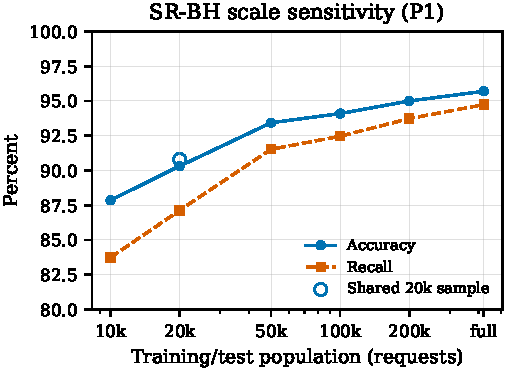
\includegraphics[width=3.4in,height=\textheight,keepaspectratio,alt={Figure 4. SR-BH scale sensitivity under P1. Accuracy and recall are plotted against the training/test population for nested subsets drawn from the full corpus at the same class prevalence. The open circle marks the separate shared 20k sample used in Table 4. The curve is monotonic, so the full-versus-20k gap is a sample-size effect, not a class-prior artefact.}]{figures/revision_srbh_learning.pdf}
\caption{SR-BH scale sensitivity under P1. Accuracy and recall
are plotted against the training/test population for nested subsets
drawn from the full corpus at the same class prevalence. The open circle
marks the separate shared 20k sample used in Table~\ref{tab:matched-operating}. The curve is
monotonic, so the full-versus-20k gap is a sample-size effect, not a
class-prior artefact.}\label{fig:learning}
\end{figure}

\subsection{v3 versus v4}\label{v3-versus-v4}

Table~\ref{tab:v3-v4} reports the nested comparison of v3 and v4 on CSIC P1 over three
seeds.



{
\begingroup\scriptsize\setlength{\tabcolsep}{3pt}
\begin{longtable}[]{@{}
  >{\raggedright\arraybackslash}p{(\linewidth - 12\tabcolsep) * \real{0.1429}}
  >{\raggedright\arraybackslash}p{(\linewidth - 12\tabcolsep) * \real{0.1429}}
  >{\raggedleft\arraybackslash}p{(\linewidth - 12\tabcolsep) * \real{0.1429}}
  >{\raggedleft\arraybackslash}p{(\linewidth - 12\tabcolsep) * \real{0.1429}}
  >{\raggedleft\arraybackslash}p{(\linewidth - 12\tabcolsep) * \real{0.1429}}
  >{\raggedleft\arraybackslash}p{(\linewidth - 12\tabcolsep) * \real{0.1429}}
  >{\raggedleft\arraybackslash}p{(\linewidth - 12\tabcolsep) * \real{0.1429}}@{}}
\caption{v3 versus v4 on CSIC 2010 (P1, three seeds). Thresholds
are selected by inner five-fold cross-validation inside each outer
training fold. Values are percentages; entries are means over seeds and
parentheses are standard deviations.}\label{tab:v3-v4}\\
\toprule\noalign{}
feature set & policy & threshold & accuracy & FPR & FNR & F1 \\
\midrule\noalign{}
\endfirsthead
\toprule\noalign{}
feature set & policy & threshold & accuracy & FPR & FNR & F1 \\
\midrule\noalign{}
\endhead
\bottomrule\noalign{}
\endlastfoot
v3 & f1 & 0.45 & 95.87 (0.14) & 3.11 (0.20) & 5.33 & 0.9548 \\
v3 & fpr1 & 0.68 & 92.17 (0.09) & 0.60 (0.03) & 16.27 & 0.9080 \\
v3 & fpr2 & 0.57 & 94.67 (0.09) & 1.26 (0.09) & 10.09 & 0.9396 \\
v4 & f1 & 0.45 & 95.91 (0.15) & 3.03 (0.24) & 5.32 & 0.9553 \\
v4 & fpr1 & 0.68 & 92.16 (0.05) & 0.58 (0.03) & 16.31 & 0.9078 \\
v4 & fpr2 & 0.57 & 94.59 (0.04) & 1.24 (0.08) & 10.27 & 0.9387 \\
\end{longtable}
\endgroup
}

Paired McNemar (seed 42, F1 policy): \(b=70\), \(c=90\), \(p=0.1328\).

\(\Delta\)accuracy (v4 \(-\) v3) = +0.06 pp (95\% bootstrap CI {[}-0.01,
+0.13{]}).

At the F1-optimal policy, v3 reaches 95.87\% at 3.11\% FPR and v4
95.91\% at 3.03\%. At FPR $\le$ 2\%, v3 reaches 94.67\% at 1.26\%
and v4 94.59\% at 1.24\%. At seed 42 and the F1 policy the paired
McNemar test gives \(p=0.1328\); the accuracy difference is +0.06 points
with a 95\% interval of {[}-0.01, +0.13{]}, not statistically
distinguishable from zero.

The cross-fitted comparison in Table~\ref{tab:matched-operating} tells the same story: both sets
reach 95.55\%; v3 has 1.94\% FPR and v4 1.96\%, and the paired
difference is -0.01 points ({[}-0.07, +0.06{]}, \(p=0.8624\)). The two
dropped features are exactly constant zero on every CSIC request, so
removing them cannot change a tree split, and the small forest
differences are RNG tie-breaking. v4 is not claimed to be more accurate
or meaningfully faster; its value is that every feature's presence or
removal is justified by recorded evidence.

\subsection{Cross-corpus transfer and direction
reversal}\label{cross-corpus-transfer-and-direction-reversal}

Ten features reverse on both independent corpora.
\texttt{hex\_\allowbreak{}encoding\_\allowbreak{}ratio} is +0.386 on CSIC but -0.537 on ECML and
-0.417 on SR-BH; \texttt{special\_\allowbreak{}char\_\allowbreak{}ratio} is +0.179 on CSIC but
-0.695 on ECML. A feature can be stable across two corpora and reverse
on a third, so two corpora are not enough to establish universality.

The reversal is not a threshold problem: the direction of the
feature-label relationship changes, so a model that learned a positive
coefficient on CSIC will rank SR-BH attacks below clean requests on that
feature. CSIC to ECML reaches 37.93\% accuracy at 86.02\% FPR; CSIC to
OpenAppSec 39.43\% at 88.80\%; SR-BH to CSIC 63.06\% at 21.72\%. The
ROC-AUCs tell the deeper story: CSIC to SR-BH is 0.435 and SR-BH to ECML
is 0.486, both below chance. A below-chance AUC cannot be fixed by
moving the threshold; the ranking itself is inverted. The remedies are
local retraining, local feature selection, or a representation invariant
across populations.

\subsection{Inline latency and ONNX
parity}\label{inline-latency-and-onnx-parity}

Table~\ref{tab:latency} reports the end-to-end latency. The measured path includes Node
extraction, JSON serialisation, HTTP transport to the Python service,
ONNX inference, threat typing, and the verdict. It excludes synchronous
SQLite writes, disk logging, and containment side effects.



{
\begingroup\scriptsize\setlength{\tabcolsep}{2pt}
\begin{longtable}[]{@{}
  >{\raggedright\arraybackslash}p{(\linewidth - 14\tabcolsep) * \real{0.0968}}
  >{\raggedleft\arraybackslash}p{(\linewidth - 14\tabcolsep) * \real{0.1290}}
  >{\raggedleft\arraybackslash}p{(\linewidth - 14\tabcolsep) * \real{0.1290}}
  >{\raggedleft\arraybackslash}p{(\linewidth - 14\tabcolsep) * \real{0.1290}}
  >{\raggedleft\arraybackslash}p{(\linewidth - 14\tabcolsep) * \real{0.1290}}
  >{\raggedleft\arraybackslash}p{(\linewidth - 14\tabcolsep) * \real{0.1290}}
  >{\raggedleft\arraybackslash}p{(\linewidth - 14\tabcolsep) * \real{0.1290}}
  >{\raggedleft\arraybackslash}p{(\linewidth - 14\tabcolsep) * \real{0.1290}}@{}}
\caption{End-to-end inline latency over 10,000 real requests
(300 warm-up, 9,700 measured, zero failures). Extraction, score, and
HTTP columns are p95; total columns are p50/p95/p99. All values are
milliseconds. The 5 ms line is a reference point, not a pass/fail
target.}\label{tab:latency}\\
\toprule\noalign{}
\begin{minipage}[t]{\linewidth}\raggedright
corpus
\end{minipage} & \begin{minipage}[t]{\linewidth}\raggedleft
n
\end{minipage} & \begin{minipage}[t]{\linewidth}\raggedleft
extraction p95
\end{minipage} & \begin{minipage}[t]{\linewidth}\raggedleft
score p95
\end{minipage} & \begin{minipage}[t]{\linewidth}\raggedleft
HTTP p95
\end{minipage} & \begin{minipage}[t]{\linewidth}\raggedleft
total p50
\end{minipage} & \begin{minipage}[t]{\linewidth}\raggedleft
total p95
\end{minipage} & \begin{minipage}[t]{\linewidth}\raggedleft
total p99
\end{minipage} \\
\midrule\noalign{}
\endfirsthead
\toprule\noalign{}
\begin{minipage}[t]{\linewidth}\raggedright
corpus
\end{minipage} & \begin{minipage}[t]{\linewidth}\raggedleft
n
\end{minipage} & \begin{minipage}[t]{\linewidth}\raggedleft
extraction p95
\end{minipage} & \begin{minipage}[t]{\linewidth}\raggedleft
score p95
\end{minipage} & \begin{minipage}[t]{\linewidth}\raggedleft
HTTP p95
\end{minipage} & \begin{minipage}[t]{\linewidth}\raggedleft
total p50
\end{minipage} & \begin{minipage}[t]{\linewidth}\raggedleft
total p95
\end{minipage} & \begin{minipage}[t]{\linewidth}\raggedleft
total p99
\end{minipage} \\
\midrule\noalign{}
\endhead
\bottomrule\noalign{}
\endlastfoot
csic & 4,700 & 0.177 & 0.003 & 3.719 & 2.911 & 3.862 & 5.860 \\
ecml & 3,000 & 0.183 & 0.004 & 3.395 & 2.791 & 3.540 & 5.343 \\
wcp & 2,000 & 0.334 & 0.004 & 3.539 & 2.886 & 3.848 & 5.739 \\
all & 9,700 & 0.197 & 0.004 & 3.614 & 2.863 & 3.779 & 5.692 \\
\end{longtable}
\endgroup
}

The overall p50 is 2.86 ms, p95 is 3.78 ms, and p99 is 5.69 ms. The HTTP
hop dominates: its p95 is 3.61 ms, while extraction is 0.20 ms and ONNX
scoring is 0.004 ms. A p95 is not a guarantee that one request in a
hundred will not exceed 5 ms: the measured p99 is 5.69 ms, and the 8 KiB
adversarial extraction worst case is 6.68 ms p95. A hard bound below
that tail would need a persistent connection, a co-located inference
library, or batching.

A separate same-machine microbenchmark isolates the 22-D to 20-D
difference on the same 10,000 frozen inputs, with 300 warm-up requests
and the median of three passes. Python extraction p95 is 0.54 ms for v3
and 0.49 ms for a benchmark-only 20-D path that skips the two dropped
features (\(\Delta = -0.05\) ms); single-threaded ONNX inference p95 is
0.46 ms for the shipped 22-D gate and 0.47 ms for a 20-D forest trained
only for timing (\(\Delta = +0.02\) ms). The 20-D model is not an
accuracy artifact, and the differences are within run-to-run noise. v4
is not claimed to be meaningfully faster.

\begin{figure}
\centering
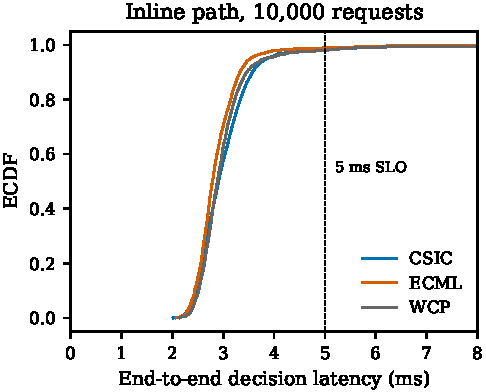
\includegraphics[width=3.4in,height=\textheight,keepaspectratio,alt={Figure 5. ECDF of end-to-end latency for the three input corpora. The dashed line marks 5 ms for reference. The curves cross it near the 95th percentile; the tail beyond 5 ms is visible.}]{figures/latency_ecdf.pdf}
\caption{ECDF of end-to-end latency for the three input
corpora. The dashed line marks 5 ms for reference. The curves cross it
near the 95th percentile; the tail beyond 5 ms is
visible.}\label{fig:latency}
\end{figure}

The ONNX parity check covers 79,593 records. The maximum absolute
probability difference between the joblib and ONNX gates is
\(1.79 \times 10^{-7}\). There are three label disagreements, all at
probability ties, and zero non-tie disagreements. The threat-typing
model has a maximum difference of \(1.26 \times 10^{-7}\) and 1,022
label mismatches, all ties, with zero non-tie mismatches. The check does
not cover the JavaScript extractor; a full cross-language feature parity
test would be stronger and is noted as a limitation.

\section{Baselines, CRS paranoia, fusion, and adversarial
evaluation}\label{baselines-crs-paranoia-fusion-and-adversarial-evaluation}

\subsection{CRS paranoia levels}\label{crs-paranoia-levels}

Table~\ref{tab:crs} reports the same 34,593 CSIC requests replayed through CRS at
paranoia levels 1, 2, and 3. The inbound anomaly threshold is 5,
request-body inspection is on, response-body inspection is off, and the
origin returns HTTP 200. A 403 is a block and a 200 an allow; edge
rejections (400/405/413/414) are excluded from the decision metrics.



{
\begingroup\fontsize{7}{8.4}\selectfont\setlength{\tabcolsep}{2pt}
\begin{longtable}[]{@{}
  >{\raggedleft\arraybackslash}p{(\linewidth - 18\tabcolsep) * \real{0.1000}}
  >{\raggedleft\arraybackslash}p{(\linewidth - 18\tabcolsep) * \real{0.1000}}
  >{\raggedleft\arraybackslash}p{(\linewidth - 18\tabcolsep) * \real{0.1000}}
  >{\raggedleft\arraybackslash}p{(\linewidth - 18\tabcolsep) * \real{0.1000}}
  >{\raggedleft\arraybackslash}p{(\linewidth - 18\tabcolsep) * \real{0.1000}}
  >{\raggedleft\arraybackslash}p{(\linewidth - 18\tabcolsep) * \real{0.1000}}
  >{\raggedleft\arraybackslash}p{(\linewidth - 18\tabcolsep) * \real{0.1000}}
  >{\raggedleft\arraybackslash}p{(\linewidth - 18\tabcolsep) * \real{0.1000}}
  >{\raggedleft\arraybackslash}p{(\linewidth - 18\tabcolsep) * \real{0.1000}}
  >{\raggedleft\arraybackslash}p{(\linewidth - 18\tabcolsep) * \real{0.1000}}@{}}
\caption{ModSecurity CRS paranoia levels on CSIC 2010. The same
requests are replayed at PL1, PL2, and PL3. The inbound anomaly
threshold is 5. Edge rejections (HTTP 400/405/413/414) and transport
failures (status 0) are excluded from the decision metrics. Each level
is a frozen configuration, not a tuned operating point. Values are
percentages except the p95 latency column, which is milliseconds.}\label{tab:crs}\\
\toprule\noalign{}
\begin{minipage}[t]{\linewidth}\raggedleft
paranoia level
\end{minipage} & \begin{minipage}[t]{\linewidth}\raggedleft
accuracy
\end{minipage} & \begin{minipage}[t]{\linewidth}\raggedleft
FPR
\end{minipage} & \begin{minipage}[t]{\linewidth}\raggedleft
recall
\end{minipage} & \begin{minipage}[t]{\linewidth}\raggedleft
F1
\end{minipage} & \begin{minipage}[t]{\linewidth}\raggedleft
TP
\end{minipage} & \begin{minipage}[t]{\linewidth}\raggedleft
TN
\end{minipage} & \begin{minipage}[t]{\linewidth}\raggedleft
FP
\end{minipage} & \begin{minipage}[t]{\linewidth}\raggedleft
FN
\end{minipage} & \begin{minipage}[t]{\linewidth}\raggedleft
p95 latency (ms)
\end{minipage} \\
\midrule\noalign{}
\endfirsthead
\toprule\noalign{}
\begin{minipage}[t]{\linewidth}\raggedleft
paranoia level
\end{minipage} & \begin{minipage}[t]{\linewidth}\raggedleft
accuracy
\end{minipage} & \begin{minipage}[t]{\linewidth}\raggedleft
FPR
\end{minipage} & \begin{minipage}[t]{\linewidth}\raggedleft
recall
\end{minipage} & \begin{minipage}[t]{\linewidth}\raggedleft
F1
\end{minipage} & \begin{minipage}[t]{\linewidth}\raggedleft
TP
\end{minipage} & \begin{minipage}[t]{\linewidth}\raggedleft
TN
\end{minipage} & \begin{minipage}[t]{\linewidth}\raggedleft
FP
\end{minipage} & \begin{minipage}[t]{\linewidth}\raggedleft
FN
\end{minipage} & \begin{minipage}[t]{\linewidth}\raggedleft
p95 latency (ms)
\end{minipage} \\
\midrule\noalign{}
\endhead
\bottomrule\noalign{}
\endlastfoot
PL1 & 66.24 & 0.03 & 26.84 & 0.4230 & 4,281 & 18,634 & 6 & 11,672 &
317.7 \\
PL2 & 63.82 & 16.07 & 40.35 & 0.5072 & 6,431 & 15,615 & 2,990 & 9,508 &
1729.8 \\
PL3 & 51.91 & 71.21 & 78.92 & 0.6021 & 12,587 & 5,366 & 13,272 & 3,362 &
1877.0 \\
\end{longtable}
\endgroup
}

Note: HTTP status counts were PL1 200: 30,306, 403: 4,287; PL2 0: 49,
200: 25,123, 403: 9,421; PL3 0: 6, 200: 8,728, 403: 25,859. Status 0 is
a transport failure; 200 is an allow and 403 is a block.

At PL1, CRS reaches 66.24\% accuracy at 0.03\% FPR with 26.84\% recall.
PL2 gives 63.82/16.07/40.35 and PL3 gives 51.91/71.21/78.92. From PL1 to
PL3 the configuration buys 52.08 points of recall at a cost of 71.18
points of FPR. PL3 flags seven in ten legitimate requests; PL2 still
exceeds the 2\% budget by a factor of eight. The paranoia level is a
recall/false-positive dial, not a substitute for a learned payload
model.

\subsection{Gate plus signature
fusion}\label{gate-plus-signature-fusion}

OR and AND fusion of the NATRIX gate and the frozen CRS replay treats
CRS as the stand-in for the Threat Intelligence role. On CSIC, OR adds
14 attacks for 6 clean false positives: recall rises by 0.09 points and
FPR by 0.03 points, and the accuracy change is not significant
(\(p=0.115\)). The CRS true positives are almost a subset of the gate's,
so the signature channel is redundant; AND is much worse, with recall
falling to 26.75\% because it is essentially the CRS decision.

On ECML, OR adds 1,483 attacks for 6,835 clean false positives (FPR
1.67\% to 21.19\%); on SR-BH, 653 for 1,463 (1.96\% to 27.16\%); on WCP,
22 for 860 (0.11\% to 6.71\%). At a 2\% budget the signature channel
either adds almost nothing or buys recall at three to twenty-five times
the budget. This is a negative result for the
gate-plus-threat-intelligence claim, and the paper reports it rather
than presenting the OR recall gain in isolation.

\subsection{Score-level fusion}\label{score-level-fusion}

The negative CRS result does not rule out fusion with a complementary
learned channel. A two-feature logistic stacker on the out-of-fold
scores of NATRIX and the lexical baseline improves on the lexical
baseline on CSIC (98.45\% versus 96.57\%, McNemar \(p<0.001\)), ECML
(94.04\% versus 93.93\%, \(p=0.0004\)), and SR-BH (96.81\% versus
95.41\%, \(p<0.001\)). On WCP it does not: 99.95\% versus 99.97\%,
\(p=0.581\), because the corpus is already near ceiling for both
detectors.

The CSIC gain survives a fully nested check: the outer five folds are
held out, the base scores are produced by an inner four-fold procedure,
and the stacker and threshold are fitted only inside the outer training
folds. The nested result is 98.24\% accuracy at 1.32\% FPR with 97.72\%
recall, so the gain is not a threshold-selection artifact. The caveats
matter. The lexical agent is not in the shipped proxy, so this is
offline headroom. The threshold is still selected by cross-fitting, not
by a fully nested procedure on every corpus. The gain is not universal:
on CSIC P2 full the stack is worse than lexical alone, on CSIC P2
payload it is tied, and on SR-BH P2 payload the apparent gain is the
NATRIX path signal re-entering the stack.

\subsection{Dilution, mutation, and the v3-D
variant}\label{dilution-mutation-and-the-v3-d-variant}

Table~\ref{tab:dilution} reports the dilution analysis. The bounded suite applies the
full mutation set to all 15,953 CSIC attacks. The targeted subset
appends a 48-character ignored probe parameter to every attack that has
a query or body (14,350 of 15,953); it is the operator that the
aggregate-ratio features are most exposed to. The v3-D variant adds nine
per-parameter and per-path maxima to the 22-D contract:
\texttt{max\_\allowbreak{}value\_\allowbreak{}digit\_\allowbreak{}ratio},
\texttt{max\_\allowbreak{}value\_\allowbreak{}uppercase\_\allowbreak{}ratio}, \texttt{max\_\allowbreak{}value\_\allowbreak{}entropy},
\texttt{max\_\allowbreak{}value\_\allowbreak{}hex\_\allowbreak{}ratio}, \texttt{max\_\allowbreak{}value\_\allowbreak{}keyword\_\allowbreak{}score},
\texttt{path\_\allowbreak{}special\_\allowbreak{}char\_\allowbreak{}ratio}, \texttt{path\_\allowbreak{}digit\_\allowbreak{}ratio},
\texttt{path\_\allowbreak{}uppercase\_\allowbreak{}ratio}, and \texttt{path\_\allowbreak{}keyword\_\allowbreak{}score}.



\needspace{9\baselineskip}
\textbf{Panel A: bounded mutation suite (all 15,953 attacks)}

{
\begingroup\scriptsize\setlength{\tabcolsep}{3pt}
\begin{longtable}[]{@{}
  >{\raggedright\arraybackslash}p{(\linewidth - 12\tabcolsep) * \real{0.1111}}
  >{\raggedleft\arraybackslash}p{(\linewidth - 12\tabcolsep) * \real{0.1481}}
  >{\raggedleft\arraybackslash}p{(\linewidth - 12\tabcolsep) * \real{0.1481}}
  >{\raggedleft\arraybackslash}p{(\linewidth - 12\tabcolsep) * \real{0.1481}}
  >{\raggedleft\arraybackslash}p{(\linewidth - 12\tabcolsep) * \real{0.1481}}
  >{\raggedleft\arraybackslash}p{(\linewidth - 12\tabcolsep) * \real{0.1481}}
  >{\raggedleft\arraybackslash}p{(\linewidth - 12\tabcolsep) * \real{0.1481}}@{}}
\caption{Dilution-resistant feature variant (v3-D). Panel A is
the bounded mutation suite over all 15,953 attacks. Panel B is the
targeted dilution subset. Panel C is the per-operator loss for the
bounded suite. Values are percentages except the evaded count.}\label{tab:dilution}\\
\toprule\noalign{}
\begin{minipage}[t]{\linewidth}\raggedright
contract
\end{minipage} & \begin{minipage}[t]{\linewidth}\raggedleft
clean accuracy
\end{minipage} & \begin{minipage}[t]{\linewidth}\raggedleft
clean FPR
\end{minipage} & \begin{minipage}[t]{\linewidth}\raggedleft
clean recall
\end{minipage} & \begin{minipage}[t]{\linewidth}\raggedleft
mutated recall
\end{minipage} & \begin{minipage}[t]{\linewidth}\raggedleft
delta (pp)
\end{minipage} & \begin{minipage}[t]{\linewidth}\raggedleft
evaded
\end{minipage} \\
\midrule\noalign{}
\endfirsthead
\toprule\noalign{}
\begin{minipage}[t]{\linewidth}\raggedright
contract
\end{minipage} & \begin{minipage}[t]{\linewidth}\raggedleft
clean accuracy
\end{minipage} & \begin{minipage}[t]{\linewidth}\raggedleft
clean FPR
\end{minipage} & \begin{minipage}[t]{\linewidth}\raggedleft
clean recall
\end{minipage} & \begin{minipage}[t]{\linewidth}\raggedleft
mutated recall
\end{minipage} & \begin{minipage}[t]{\linewidth}\raggedleft
delta (pp)
\end{minipage} & \begin{minipage}[t]{\linewidth}\raggedleft
evaded
\end{minipage} \\
\midrule\noalign{}
\endhead
\bottomrule\noalign{}
\endlastfoot
v3 & 95.55 & 1.93 & 92.60 & 82.47 & -10.13 & 2,639 \\
v3-D & 96.79 & 2.08 & 95.46 & 85.51 & -9.95 & 2,222 \\
\end{longtable}
\endgroup
}

\needspace{9\baselineskip}
\textbf{Panel B: targeted dilution subset}

{\def\LTcaptype{none} % do not increment counter
\begingroup\small
\noindent\begin{tabular}{@{}
  >{\raggedright\arraybackslash}p{(\linewidth - 8\tabcolsep) * \real{0.2000}}
  >{\raggedleft\arraybackslash}p{(\linewidth - 8\tabcolsep) * \real{0.2000}}
  >{\raggedleft\arraybackslash}p{(\linewidth - 8\tabcolsep) * \real{0.2000}}
  >{\raggedleft\arraybackslash}p{(\linewidth - 8\tabcolsep) * \real{0.2000}}
  >{\raggedleft\arraybackslash}p{(\linewidth - 8\tabcolsep) * \real{0.2000}}@{}}
\toprule
contract & original recall & mutated recall & delta (pp) & evaded \\
\midrule
v3 & 91.83 & 58.51 & -33.32 & 5,197 \\
v3-D & 94.99 & 66.55 & -28.44 & 4,387 \\
\bottomrule
\end{tabular}
\endgroup
}

\needspace{9\baselineskip}
\textbf{Panel C: per-operator loss (bounded suite)}

{\def\LTcaptype{none} % do not increment counter
\begingroup\scriptsize\setlength{\tabcolsep}{2pt}
\noindent\begin{tabular}{@{}
  >{\raggedright\arraybackslash}p{(\linewidth - 10\tabcolsep) * \real{0.2000}}
  >{\raggedleft\arraybackslash}p{(\linewidth - 10\tabcolsep) * \real{0.1400}}
  >{\raggedleft\arraybackslash}p{(\linewidth - 10\tabcolsep) * \real{0.1700}}
  >{\raggedleft\arraybackslash}p{(\linewidth - 10\tabcolsep) * \real{0.1700}}
  >{\raggedleft\arraybackslash}p{(\linewidth - 10\tabcolsep) * \real{0.1600}}
  >{\raggedleft\arraybackslash}p{(\linewidth - 10\tabcolsep) * \real{0.1600}}@{}}
\toprule
operator
 & n
 & v3 delta (pp)
 & v3-D delta (pp)
 & v3 evaded
 & v3-D evaded
 \\
\midrule
case & 621 & -0.64 & -2.90 & 16 & 22 \\
sql\_comment & 72 & +0.00 & -13.89 & 0 & 10 \\
double\_encode & 12,602 & -2.86 & -0.37 & 1,325 & 678 \\
dilution & 14,338 & -11.27 & -11.07 & 2,639 & 2,221 \\
\bottomrule
\end{tabular}
\endgroup
}

The clean contract reaches 95.55\% accuracy at 1.93\% FPR with 92.60\%
recall; under bounded mutation its recall falls to 82.47\% (\(-10.13\)
points), and 2,639 of the 14,773 attacks that NATRIX originally blocked
are evaded (17.86\% of blocked attacks). v3-D reaches 96.79\% accuracy
at 2.08\% FPR with 95.46\% clean recall; under bounded mutation its
recall falls to 85.51\% (\(-9.95\) points), and 2,222 attacks are
evaded. The targeted subset is harsher: v3 falls from 91.83\% to 58.51\%
(\(-33.32\) points, 5,197 evaded), while v3-D falls from 94.99\% to
66.55\% (\(-28.44\) points, 4,387 evaded). The targeted loss is 4.88
points smaller for v3-D, but it is still a 28-point loss. The fix is
partial.

The per-operator panel explains why. Dilution costs v3 11.27 points and
v3-D 11.07: the per-parameter maxima do not remove the dilution effect,
because an ignored parameter still changes request length and the
aggregate ratios that are not replaced by a maximum. Double encoding
costs v3 2.86 points but v3-D only 0.37, which is the improvement the
variant was designed for. The variant also introduces new weaknesses:
case changes cost v3 0.64 points but v3-D 2.90, and SQL-comment
insertion is neutral for v3 but costs v3-D 13.89 points on the
72-request subgroup. The paper reports the trade-off rather than
claiming a uniform robustness gain.

CRS behaves differently on the same mutated requests. Its recall falls
only from 26.84\% to 26.05\% (\(-0.79\) points), and only 2.94\% of its
blocked attacks are evaded, but it starts from far lower recall: the
absolute number of detected attacks falls by 126, while NATRIX loses
2,639. The operator breakdown shows genuine complementarity: dilution
costs NATRIX 11.27 points but CRS only 0.84, and double encoding costs
NATRIX 2.86 points but CRS 0.82; in the other direction, SQL-comment
insertion evades 44 of 44 originally blocked CRS attacks in a 72-request
subgroup while NATRIX is unaffected, and case changes cost CRS 4.51
points but NATRIX 0.64. Neither detector dominates. The test is bounded
and deterministic: it is not an adaptive search, the mutation budget is
at most three operators, and a mutated payload is not guaranteed to
remain exploitable.

\subsection{WCP 2024 as a diagnostic}\label{wcp-2024-as-a-diagnostic}

WCP is the newest corpus and the clearest example of a benchmark
artifact. Every one of the 73,924 malicious requests has path
\texttt{/\allowbreak{}}, while the 137,820 legitimate requests span thousands of
paths from 692 sites. On the random 20k split, an endpoint-only lexical
model reaches 100\% recall at 1.31\% FPR, and NATRIX reaches 99.79\%
accuracy.

Restricting to requests whose path is exactly \texttt{/\allowbreak{}} leaves 170
clean and 6,982 attack rows. NATRIX blocks 0 of the 170 clean rows
(Wilson 95\% upper bound 2.21\%) and 99.64\% of attacks. The lexical
full and payload views reach 99.91\% and 99.89\% recall with 0 false
positives; CRS reaches 88.80\% recall at 24.12\% FPR; the endpoint-only
model collapses to 100\% FPR, confirming that the random-split result
was an endpoint artifact. The clean subset is small, the payloads are
easy, and the legitimate traffic is site-clustered, so this is a
diagnostic, not a generalisation claim.

\section{Formal verification}\label{formal-verification}

The formal claim is about control flow and trust arithmetic, not about
whether the protocol chooses good rules, whether the canary sample is
representative, or whether the agents are independent in a Byzantine
sense. The TLA+ specification \citep{lamport2002specifying}
\texttt{Cppp.\allowbreak{}tla} models three agents, a set of rules, a quorum \(K=2\),
a trust floor \(\tau=2\), and a maximum trust of 3. The Python reference
\texttt{cppp.\allowbreak{}py} mirrors the TLA+ guards, and the property suite
\texttt{test\_\allowbreak{}formal.\allowbreak{}py} contains 13 tests, all passing. The
breadth-first enumeration is bounded at depth 9 and is not a proof for
unbounded executions, but it exercises the implementation rather than
only the specification. The mutation test removes one guard at a time
and asks TLC whether the corresponding invariant is violated; all eight
mutants are killed, which shows that the invariants are sensitive to the
transitions they constrain. The trust-decay verification checks
boundedness, monotone decay, the half-life definition, recovery bounds,
the closed form, and convergence over 81,484 exact-rational cases; a
floating-point grid would introduce tolerance decisions and could hide a
violation near the boundary. The sidecar over 916 audit records verified
the hash chain, matched 108 promotions with 108 retirements (8
automatic), and held all eight invariants; its full cycle cost 33.75 ms
p95, with validation the operation to move off the critical path.

\section{Deployment audit and the enforcement
boundary}\label{deployment-audit-and-the-enforcement-boundary}

CPPP is only useful if it can be applied to a real promotion decision,
so we audited the existing deployment rather than building a new one.
The gateway runs on Render, the SOC dashboard on Vercel, and the
protected origin is a public portfolio reached through a path-scoped
route. The audit has three parts: a repeated labelled probe suite, the
gate's own decision ledger, and an offline replay of the predicate that
actually enforces.

\textbf{Labelled probe suite.} Each run sends ten benign requests first
(home page, campaign query, two SPA routes, static bundles, search,
pagination, an apostrophe, an email parameter) and then ten attacks (SQL
injection, reflected and evasive XSS, traversal, command injection,
null-byte extension bypass, double encoding, scanner path, Log4Shell).
Benign-first ordering prevents an attack-triggered adaptive block from
contaminating the false-positive count. Three runs, 20 s apart, each
returned TP=10, FP=0, TN=10, FN=0, and each rendered the origin's
portfolio title; pooled over 60 probes, 30/30 attacks were blocked and
0/30 benign requests were blocked. This is a policy check on a fixed
probe set, not a generalisation estimate.

\textbf{What the gate actually decides.} Only 33 of the 60 probes
produced a gate decision. The other 27 were handled before the gate: two
static bundles per run were served without a decision, and 21 attacks
were blocked by the lexical rule layer. The gate ledger is nonetheless
unambiguous. All 24 benign requests that reached it were scored as
attacks, with probabilities from 0.75 to 1.00, and all 24 were marked
inapplicable and allowed. All 9 attacks that reached it were scored
above threshold and enforced. The gate is therefore not a calibrated
detector on this traffic; it is a corroborator. Enforcement is the
conjunction of the score with an independent lexical predicate
(\texttt{gate\allowbreak{}Has\allowbreak{}Lexical\allowbreak{}Signal}): null byte, command injection, SQL, XSS,
traversal, hexadecimal ratio above 0.2, or a suspicious extension.
Inference on the audit rows took 0.23--0.45 ms (median 0.30 ms), so the
model is cheap; the decision that produces the zero-FP result is the
predicate, not the score.

\textbf{The cost of the conjunction.} Table~\ref{tab:deployment} replays the predicate on
the labelled corpora at the deployed threshold of 0.5. On CSIC P1 the
model alone reaches 92.94\% recall at 2.07\% FPR; the conjunction gives
34.66\% recall at 0.00\% FPR. The same pattern holds under P2
(89.82/24.30 to 34.41/5.64), on ECML P1 (76.96/1.50 to 53.47/0.68), and
on the SR-BH 20k sample (96.24/10.92 to 59.36/1.43). The predicate buys
false-positive suppression by discarding most of the detector's recall.
It is a deployment guard, not evidence that the model is calibrated, and
it cannot be audited as a detector.



{
\begingroup\fontsize{7}{8.4}\selectfont\setlength{\tabcolsep}{2pt}
\begin{longtable}[]{@{}
  >{\raggedright\arraybackslash}p{(\linewidth - 18\tabcolsep) * \real{0.1062}}
  >{\raggedright\arraybackslash}p{(\linewidth - 18\tabcolsep) * \real{0.0708}}
  >{\raggedright\arraybackslash}p{(\linewidth - 18\tabcolsep) * \real{0.0973}}
  >{\raggedright\arraybackslash}p{(\linewidth - 18\tabcolsep) * \real{0.1062}}
  >{\raggedright\arraybackslash}p{(\linewidth - 18\tabcolsep) * \real{0.0973}}
  >{\raggedright\arraybackslash}p{(\linewidth - 18\tabcolsep) * \real{0.0973}}
  >{\raggedright\arraybackslash}p{(\linewidth - 18\tabcolsep) * \real{0.1150}}
  >{\raggedright\arraybackslash}p{(\linewidth - 18\tabcolsep) * \real{0.0973}}
  >{\raggedright\arraybackslash}p{(\linewidth - 18\tabcolsep) * \real{0.0973}}
  >{\raggedright\arraybackslash}p{(\linewidth - 18\tabcolsep) * \real{0.1150}}@{}}
\caption{Deployed enforcement boundary at threshold 0.5.
\texttt{Pred.\allowbreak{}} is the \texttt{gate\allowbreak{}Has\allowbreak{}Lexical\allowbreak{}Signal} predicate replayed
offline; \texttt{Model} uses the score alone; \texttt{Conj.\allowbreak{}} requires
both. Values are percentages except the corpus and split columns.}\label{tab:deployment}\\
\toprule\noalign{}
\begin{minipage}[t]{\linewidth}\raggedright
Corpus
\end{minipage} & \begin{minipage}[t]{\linewidth}\raggedright
Split
\end{minipage} & \begin{minipage}[t]{\linewidth}\raggedright
Pred. clean
\end{minipage} & \begin{minipage}[t]{\linewidth}\raggedright
Pred. attack
\end{minipage} & \begin{minipage}[t]{\linewidth}\raggedright
Model acc
\end{minipage} & \begin{minipage}[t]{\linewidth}\raggedright
Model FPR
\end{minipage} & \begin{minipage}[t]{\linewidth}\raggedright
Model recall
\end{minipage} & \begin{minipage}[t]{\linewidth}\raggedright
Conj. acc
\end{minipage} & \begin{minipage}[t]{\linewidth}\raggedright
Conj. FPR
\end{minipage} & \begin{minipage}[t]{\linewidth}\raggedright
Conj. recall
\end{minipage} \\
\midrule\noalign{}
\endfirsthead
\toprule\noalign{}
\begin{minipage}[t]{\linewidth}\raggedright
Corpus
\end{minipage} & \begin{minipage}[t]{\linewidth}\raggedright
Split
\end{minipage} & \begin{minipage}[t]{\linewidth}\raggedright
Pred. clean
\end{minipage} & \begin{minipage}[t]{\linewidth}\raggedright
Pred. attack
\end{minipage} & \begin{minipage}[t]{\linewidth}\raggedright
Model acc
\end{minipage} & \begin{minipage}[t]{\linewidth}\raggedright
Model FPR
\end{minipage} & \begin{minipage}[t]{\linewidth}\raggedright
Model recall
\end{minipage} & \begin{minipage}[t]{\linewidth}\raggedright
Conj. acc
\end{minipage} & \begin{minipage}[t]{\linewidth}\raggedright
Conj. FPR
\end{minipage} & \begin{minipage}[t]{\linewidth}\raggedright
Conj. recall
\end{minipage} \\
\midrule\noalign{}
\endhead
\bottomrule\noalign{}
\endlastfoot
CSIC & P1 & 20.5\% & 34.7\% & 95.63 & 2.07 & 92.94 & 69.87 & 0.00 &
34.66 \\
CSIC & P2 & 20.5\% & 34.7\% & 82.21 & 24.30 & 89.82 & 66.72 & 5.64 &
34.41 \\
ECML & P1 & 21.8\% & 59.8\% & 92.00 & 1.50 & 76.96 & 85.50 & 0.68 &
53.47 \\
ECML & P2 & 21.8\% & 59.8\% & 91.65 & 1.50 & 75.76 & 85.44 & 0.67 &
53.24 \\
SR-BH 20k & P1 & 33.4\% & 59.8\% & 94.16 & 10.92 & 96.24 & 70.75 & 1.43
& 59.36 \\
SR-BH 20k & P2 & 33.4\% & 59.8\% & 92.92 & 14.84 & 96.09 & 70.68 & 1.50
& 59.30 \\
\end{longtable}
\endgroup
}

\textbf{Canary counterfactual.} A gate decision is a promotion decision
in miniature. Treat the eight benign requests that reached the gate in
one run as a canary sample for a candidate that fires whenever the score
is at least 0.5. The candidate records eight observations and eight
hits. In the evidence-coupled CPPP, \texttt{Pass\allowbreak{}Canary} requires
\texttt{canarySeen\ \textgreater{}=\ N} and \texttt{canary\allowbreak{}Hits\ =\ 0},
and \texttt{No\allowbreak{}Promotion\allowbreak{}With\allowbreak{}Canary\allowbreak{}Hit} makes a hit permanent; the rule is
refused. The shipped proxy instead inserts a learned signature with
\texttt{hit\allowbreak{}Count\ =\ 1} and activates it when
\texttt{hitCount\ \textgreater{}=\ 2}, with no benign-evidence test. The
audit therefore exhibits on live traffic the exact shortcut that the
protocol forbids, rather than only in the model. The counterfactual does
not show that CPPP would improve accuracy; it shows that CPPP refuses a
promotion that the operator cannot justify with benign evidence.

\textbf{Scope.} The deployment is one public gateway and one origin, the
probe set is small and hand-written, and the canary sample is not
representative. The audit shows that the deployment path works and that
the enforcement boundary is real; it is not a shadow-mode trial, a
generalisation estimate, or a claim that the gate is calibrated. A later
restart reported the model as unavailable while the rule layer still
blocked the attacks, so availability is a separate operational risk. The
per-run files, pooled aggregate, and raw gate ledger are in
\texttt{experiments/\allowbreak{}results/\allowbreak{}live\_\allowbreak{}gate/\allowbreak{}}, together with the 20 probe
definitions.

\section{Discussion}\label{discussion}

The evidence supports six claims.

First, the comparison protocol is itself a contribution, and it carries
an interval: the full-versus-payload gap moves by 26.2 points on CSIC
when the split changes, against 0.7 on SR-BH, so a single-protocol
comparison cannot identify a usable detector. NATRIX is competitive with
a strong lexical baseline under P1 but does not beat it; under P2 the
ranking changes, with lexical full collapsing on CSIC while lexical
payload stays strong, and the opposite pattern on SR-BH.

Second, the deployment audit shows that the offline score and the
enforced decision are different objects. The gate scored every benign
probe that reached it as an attack, and a lexical predicate produced the
zero-false-positive result at a cost of 58.3 points of CSIC recall. An
audit that reported only the end-to-end block rate would have missed
this, and the same separation is what CPPP formalises as an evidence
requirement.

Third, the contract carries signal beyond a generic request-shape model,
and the cross-fitted stack with the lexical channel reaches 98.24\% at
1.32\% FPR on CSIC under a fully nested protocol. The gain is real but
offline, and it is protocol-dependent: on CSIC P2 full the stack is
worse than lexical alone, and the SR-BH P2 payload gain is the path
signal re-entering the stack.

Fourth, the three-gate mechanism is a reusable decision procedure, not a
trial-and-error search. It drops two features, retains 20, and produces
a written justification for every row; it screens 24 candidates, accepts
12 statistically, and admits none on measured cost. The inline path has
a measured p95 of 3.78 ms over 9,700 real requests, and the HTTP hop,
not the model, dominates; the cost gate separates marginal extraction
cost from the shared parse and transport.

Fifth, CPPP's control-flow safety is model-checked, mutation-tested, and
implemented as a reference implementation: \texttt{Seed\allowbreak{}Trust} removes
the construction artifact, eight of eight mutants are killed, and the
protocol forbids the direct promotion shortcut that the shipped proxy
still uses.

Sixth, the dilution fix is a measured partial improvement: v3-D raises
clean and mutated recall and reduces the targeted loss from 33.32 to
28.44 points, but introduces new weaknesses on case changes and
SQL-comment insertion.

The evidence does not support universal generalisation. ECML reaches
91.96\% under P1 and misses the accuracy target, and P2 fails on CSIC
(78.85\% at 6.50\% FPR) and on the 20k SR-BH sample relative to the full
corpus. Transfer is worse: two AUCs are below chance, and the OpenAppSec
false-positive rate is 88.80\% with a CSIC source. Ten features reverse
sign, so the learned boundary is population-specific. The evidence also
does not support a claim that NATRIX is state of the art, that v4
improves accuracy, that the mutation test establishes adversarial
robustness, that gate-plus-CRS fusion is useful at a 2\% budget, or that
the shipped runtime enforces CPPP.

The inline/async split is worth preserving: the five inline roles
account for the measured budget, while the four governance roles do not
affect the current verdict. Feature direction is not portable, so
cross-deployment federation needs explicit heterogeneity handling
\citep{mcmahan2017communication, kairouz2021advances}. The HTTP hop
dominates latency, so a hard bound needs a persistent connection,
co-located inference, or a Unix socket.

\section{Limitations}\label{limitations}

\textbf{Corpus age and construction.} CSIC 2010 and ECML/PKDD 2007 are
old and were generated against specific applications; their traffic does
not represent modern APIs, JSON, or cloud-native deployments. SR-BH 2020
is more modern but attack-dominant, so its prior is not a deployment
prior. WCP 2024 is the newest corpus, but its legitimate traffic is
capped at 200 requests per site and is site-clustered, and every
malicious row has path \texttt{/\allowbreak{}}; only the endpoint-matched subset is
reported. The corpora use different label ontologies, so a request
labelled attack in one corpus may be clean in another; deduplication
removes exact conflicts but not semantic ones.

\textbf{Split protocol and threshold selection.} P1 allows the same
endpoint in training and test. That is realistic for a WAF but inflates
performance relative to an unseen-endpoint deployment. P2 is the bound,
and it fails on CSIC; it removes endpoint identity but not the path
string, so it is not a payload-only protocol. The fully nested threshold
policy misses the 95\% target on CSIC by 0.33 to 0.41 points. The
cross-fitted protocol meets it, but the models that score the other
folds were trained on data that includes the held-out fold, so it is not
fully nested. The paper reports both and does not present the
cross-fitted number as frozen.

\textbf{Learner and screening configuration.} The forest is pinned to
the shipped configuration (D5), which is not tuned for these corpora. A
tuned forest might improve accuracy but would no longer be the deployed
artifact. The secondary learners are fixed untuned robustness checks,
not a model search. A single LightGBM configuration is the generic
control; a stronger control would change the comparison.

\textbf{Formal scope.} TLC checks finite constants (three agents, two
rules, \(K=2\), \(\tau=2\), max trust 3), and the BFS is bounded at
depth 9. The model does not cover Byzantine agents, Sybil identities,
model poisoning, or supply-chain compromise, and the trust values are
not calibrated to real agent reliability; it is a safety layer, not a
complete security proof.

\textbf{Latency and adversarial scope.} The benchmark is a
single-workstation component measurement. It excludes synchronous SQLite
writes, disk logging, and containment side effects, uses one Python and
one Node process, and does not measure concurrency, a load balancer, or
TLS termination. The p95 is a component result, not a service-level
guarantee. The mutation study applies a fixed, bounded set of
transformations, not an adaptive search; a mutated payload is not
guaranteed to remain exploitable, and no adversary probes the detector
for evasions \citep{biggio2018wild}.

\textbf{What evidence would settle the open claims.} The deployment
audit is 30 attack and 20 benign probes on one gateway; it shows that
the enforcement path can diverge from the score, not what the field
false-positive rate is. Three further claims need evidence this study
does not have, and each has a test that could refute it. A shadow-mode
trial that scores live traffic without enforcing, over a pre-registered
window with a labelled audit sample, a fixed FPR ceiling, and an
automatic rollback rule would settle deployment behaviour; the claim
survives only if endpoint-disjoint FPR stays within the 2\% budget and
no feature direction reverses. A query-budgeted black-box search against
the deployed gate, scored at the same 2\% FPR and compared with the
non-adaptive mutation baseline, would settle adaptive robustness. A
same-budget comparison against the strongest published WAF on a shared
corpus with endpoint-disjoint splits would settle whether the contract
is a detection advance; that claim is not made here. Until such evidence
exists, the paper claims benchmark validity and auditability only.

\textbf{Baseline, fusion, and scale comparability.} CRS is a frozen
PL1-PL3 configuration, not a detector tuned to a 2\% budget, so its rows
are not like-for-like. The lexical baseline is a standard hashed n-gram
learner and the char-CNN a self-contained reference; neither reproduces
a named system. The NATRIX+lexical stacker is offline: the lexical agent
is not in the shipped proxy, and a deployed stacker needs both scores at
request time. Only the CSIC result is repeated under a fully nested
protocol.

\section{Conclusion}\label{conclusion}

The paper's contribution is a benchmark-validity result and an audit
standard, not a new detector. The results are two-sided. On the positive
side, the full-versus-payload gap moves by 26.2 points on CSIC between
protocols with an interval that excludes zero, the deployment audit
separates the gate's score from the predicate that enforces, the
cross-fitted stack with the lexical channel reaches 98.24\% at 1.32\%
FPR under a fully nested CSIC protocol, the inline p95 is 3.78 ms over
9,700 real requests, the three-gate mechanism drops two features and
admits none of the 12 statistically accepted candidates on measured
cost, CPPP's invariants hold in TLA+ and in the executable reference,
eight of eight mutants are killed, trust decay is verified on 81,484
exact-rational cases and nine symbolic identities, and the deployed
gateway blocked 30/30 probe attacks with zero benign blocks. On the
negative side, NATRIX is not the best single detector: the lexical
full-request baseline is stronger than NATRIX at the 2\% FPR point under
P1 on all three corpora, the char-CNN is comparable on CSIC, lexical
payload is the strongest CSIC P2 detector, the fully nested policy
reaches 94.67\% and misses the 95\% target, P2 fails on CSIC (78.85\% at
6.50\% FPR), two transfer AUCs are below chance, ten features reverse
direction, gate-plus-CRS fusion is redundant or over budget, bounded
mutation removes 10.13 points of recall, and the targeted dilution
attack still removes 28.44 points with v3-D. v4 is not claimed to be
more accurate or meaningfully faster; its value is that every feature's
presence or removal is justified by recorded evidence, and WCP is
reported only as an endpoint-confounded diagnostic.

The conclusion is not that the detector is universal or state of the
art, but that the evaluation standard and the architecture are reusable.
A reported accuracy should be accompanied by the split protocol, the
feature view, and the enforcement rule that produced it. A deployment
should calibrate on local data, evaluate on endpoint-disjoint splits,
report endpoint-only and payload-only baselines, monitor feature
directions for reversal, and treat promotion as a protocol with quorum,
canary, trust, and audit. The current runtime does not yet enforce CPPP;
replacing the \texttt{hitCount\ \textgreater{}=\ 2} and import-shortcut
path is the next engineering step. Future work has five directions:
shadow-mode validation with a labelled window and rollback; adaptive
adversarial evaluation \citep{biggio2018wild}; federated learning with
local heads \citep{mcmahan2017communication, kairouz2021advances};
header-coherence features, deferred by D1; and a dilution-invariant
contract using per-parameter maxima, with a new cost-gate measurement.

\section*{Data availability}\label{data-availability}
\addcontentsline{toc}{section}{Data availability}

The datasets are public research corpora. CSIC 2010 is available from
the Information Security Institute, Spanish National Research Council.
ECML/PKDD 2007 is available from the challenge archive. SR-BH 2020 and
the OpenAppSec WAF Comparison corpus are available from their respective
public repositories. The manifest, checksums, and preprocessing counts
are in \texttt{data/\allowbreak{}manifest.\allowbreak{}json} and
\texttt{data/\allowbreak{}processed/\allowbreak{}*/\allowbreak{}*\_\allowbreak{}summary.\allowbreak{}json}. An archived copy of the code
and result files is available at
https://doi.org/10.5281/zenodo.24435601, a concept DOI that resolves to
the latest archived version. The corpora themselves are third-party and
are not redistributed; the deposit contains the manifest, checksums, and
derived result files.

\section*{Code availability}\label{code-availability}
\addcontentsline{toc}{section}{Code availability}

A reproducibility package containing the feature extractor, experiment
scripts, ONNX export, formal models, result files, and manuscript build
is available at \url{https://github.com/NameetAhire/natrix-auditable}
and archived on Zenodo \cite{natrix_artifact}. The experiment queue is
\texttt{experiments/\allowbreak{}run\_\allowbreak{}all.\allowbreak{}ps1}; the analysis plan and deviations are
in \texttt{protocol/\allowbreak{}}; the tables and figures are generated from the
result files.

\section*{Ethics statement}\label{ethics-statement}
\addcontentsline{toc}{section}{Ethics statement}

The work uses public, labelled HTTP corpora. It does not involve human
subjects, personal data collection, or live traffic interception. The
OpenAppSec legitimate sample is used only for false-positive evaluation.

\section*{CRediT author statement}\label{credit-author-statement}
\addcontentsline{toc}{section}{CRediT author statement}

\textbf{Ahire Nameet Sudam:} Conceptualization, Methodology, Software,
Formal analysis, Investigation, Data curation, Writing - original draft,
Visualization. \textbf{D. D. Ambawade:} Supervision, Methodology,
Validation, Writing - review and editing.

\section*{Declaration of competing
interest}\label{declaration-of-competing-interest}
\addcontentsline{toc}{section}{Declaration of competing interest}

The authors declare that they have no known competing financial
interests or personal relationships that could have appeared to
influence the work reported in this paper.

\section*{Declaration of generative AI and AI-assisted technologies in
the manuscript preparation
process}\label{declaration-of-generative-ai-and-ai-assisted-technologies-in-the-manuscript-preparation-process}
\addcontentsline{toc}{section}{Declaration of generative AI and
AI-assisted technologies in the manuscript preparation process}

During the preparation of this work the authors used large language
model assistants for code development, data-analysis scripting, and
manuscript editing. After using these tools, the authors reviewed and
edited the content as needed and take full responsibility for the
content of the published article.

\section*{Funding}\label{funding}
\addcontentsline{toc}{section}{Funding}

This research did not receive any specific grant from funding agencies
in the public, commercial, or not-for-profit sectors.

\section*{Acknowledgements}\label{acknowledgements}
\addcontentsline{toc}{section}{Acknowledgements}

The authors thank the maintainers of the public HTTP corpora and the
OpenAppSec project for making their data available for research.

\bibliographystyle{elsarticle-num}
\bibliography{refs}

\end{document}
